% !TEX encoding = UTF-8
% !TEX TS-program = pdflatex
% !TEX root = ../tesi.tex

%**************************************************************
\chapter{Data analysis and the outcomes}
\label{cap:data-analysis}
This chapter illustrates the analysis of the collected data, enriched by discussions and experiments.
%**************************************************************
\section{Discussions, experiments and premises about collected data analysis}
Before discussing the obtained acceptability model and describing the ``\texttt{Zero-Effort Attack}'' tool, it is necessary to pin some premises and discuss some hot spots. Thus, some small experiments carried out are cited to show how the research field is very large and full of possible paths to take.

\subsection{Number of friend request}
\label{cap:number-friend-req}
First of all, a clarification about the number of friend requests. According to the law of large numbers, with a greater amount of data collected, the result of the analyzed data is more certain and therefore more valid.
\par \noindent Thus, is correct to affirm that \texttt{3} is a small number, but it was decided thinking about the smallest exhaustive number of friend requests to do considering the available time. A greater number would have led to a greater number of logins and friend requests, actions that could have led Facebook to block profiles. With more time, logins and friend requests would be spread over time, so as not to be blocked.
\par \noindent So, \texttt{3} is the perfect number for this case of study (i.e., for the internship), because only one request not could be valued, 2 requests bring the analysis in a \textit{fifty-fifty} situation, with 3 requests one of the two possible results (friend request accepted or not) triumphs over the other.
\par \noindent It's also important to underline that the result of \textbf{the analysis is preliminary}: with more requests (but anyway the number must be odd) the model of acceptance could undergo substantial changes. Also for this reason, during the development of all tools, it has always been born in mind that they must be implemented to work with a variable amount of data.
\subsection{\texttt{victims.json} dataset: why is it so unbalanced?}
\label{cap:discuss-dataset-victims}
After the first phase of data collection, it was possible to notice that most of the users on Facebook do not enter a lot of data in their profile, making the dataset of data collected immediately very unbalanced. More precisely, few users enter their age, city of residence, and occupation (many times it is present but blatantly bogus).
\par \noindent Added to this is the fact that very few underage users who make it clear their age are very few (about 2 out of more than 1000 total profiles collected). In many cases, age can only be guessed by looking at the profile image, but this is not an evaluation criterion on which to reason. Thus, some categories contained a greater number of profiles and this caused the dataset to be very unbalanced.
\par \noindent In the first place, it was decided that these profiles were categorized anyway, but for every category, the number of profiles examined is the same. The extra profiles were useful when it was necessary to replace some victim profiles that, for some reason, could no longer be considered.
\par \noindent Then, it was decided to remove the classes of the parameters that consider the minors, and the ``\texttt{current\_town\_value}'' and ``\texttt{occupation\_value}'' parameters. All three are interesting factors to analyze in future works (details in Chapter \ref{cap:future-works}).
\subsection{Profile picture: is it really so important?}
\label{cap:discuss-image-profile}
For this project, 12 attacker profiles were created, 6 of which with a real profile image, depicting a (non-existent) person. The profile pictures were chosen consistently with the age that the corresponding attacker profile claimed to have. For example, the attacker profile ``\texttt{PF-9}'' is a 70-year-old woman and her profile picture of her represents a woman who could be said to be around that age. The value of the ``\texttt{age\_range}'' parameter of this profile is ``\texttt{3}'', as the age is greater than 50 years. In this range, however, there are also people of just 52 years and 20 years of difference are not exactly few if you wanted to make a comparison. The ``PF-9'' profile was not widely accepted, but how can one be sure that the same fate would have had a profile 20 years younger but still belonging to $\texttt{age\_value} = 3$?\par \noindent For this reason, they took some profiles with the real profile image and changed the profile image with one that, at first glance, showed a different age from the one declared (not too different of course).\par \noindent A note before showing the results: to make the change more consistent, the year of birth that the profile declares should also have been changed. With an extra profile used for testing of various kinds, this experiment was done, but Facebook took steps by blocking the profile. So, it was decided to change only the profile image, taking as good as stated in the Chapter \ref{cap:alt-technology}, or that when a user receives the friend request he is easily influenced by the profile image, so much so that many times he does not even check the true age on the appropriate page.
\par \noindent As can be seen in the Table \ref{table:change-profile-pic}, there have been some interesting results. In the first place, after changing his picture profile, \texttt{PF-5} received a friend request from a woman, the first one request for him. Then, regaring \texttt{PF-9}, after changing the profile picture to a younger woman, all three requests sent to victim profiles of type \texttt{MT2} were accepted and the same goes for the \texttt{PF-0} and the \texttt{PF-5}, where, after changing the profile picture, two women accepted the friend request. However, this did not work for the \texttt{PF-3} profile, where the profile picture changed to that of a younger man did not lead to any change in friend requests.
\par \noindent This is a small result but it wants to underline how much the profile image is therefore a valid starting point on which to deepen with a dedicated case study.
\begin{table}[H]
\begin{center}
\begin{tabular}[c]{ |c|c|m{1.5cm}|m{1.5cm}|c| } 
	\hline
	\cellcolor[HTML]{b0d7ff}\textsc{cod} & 
	\cellcolor[HTML]{b0d7ff}\textsc{label} & 
	\multicolumn{1}{|c|}{\cellcolor[HTML]{b0d7ff}\textsc{old img}}&
	\multicolumn{1}{|c|}{\cellcolor[HTML]{b0d7ff}\textsc{new img}}&
	\cellcolor[HTML]{b0d7ff}\textsc{friend request accepted}\\
	%\cellcolor[HTML]{e6f2ff}
	\hline 
	\cellcolor[HTML]{b0d7ff}\texttt{PF-9}
	&\cellcolor[HTML]{e6f2ff}\texttt{FT3}
	&\vspace{.15cm}	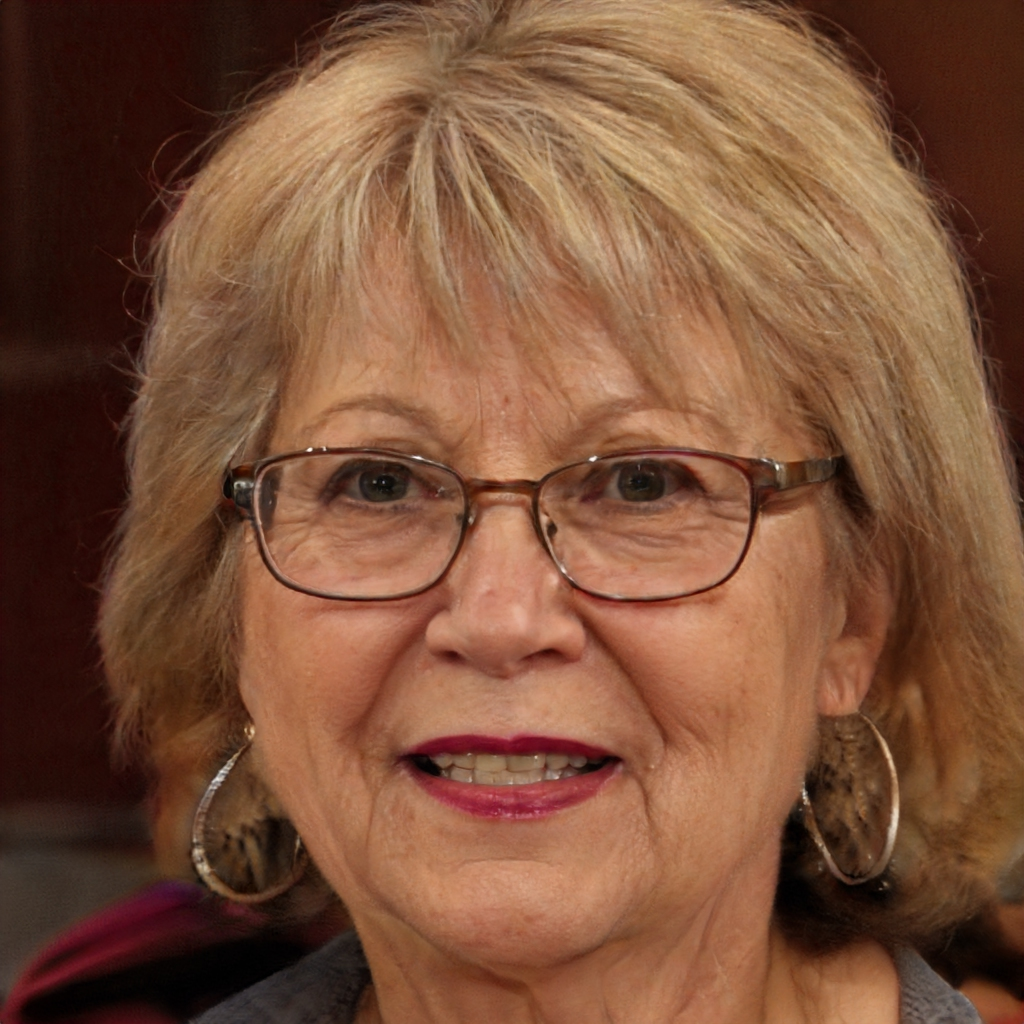
\includegraphics[height=1.5cm]{immagini/FT3.jpg}
	&\vspace{.15cm}	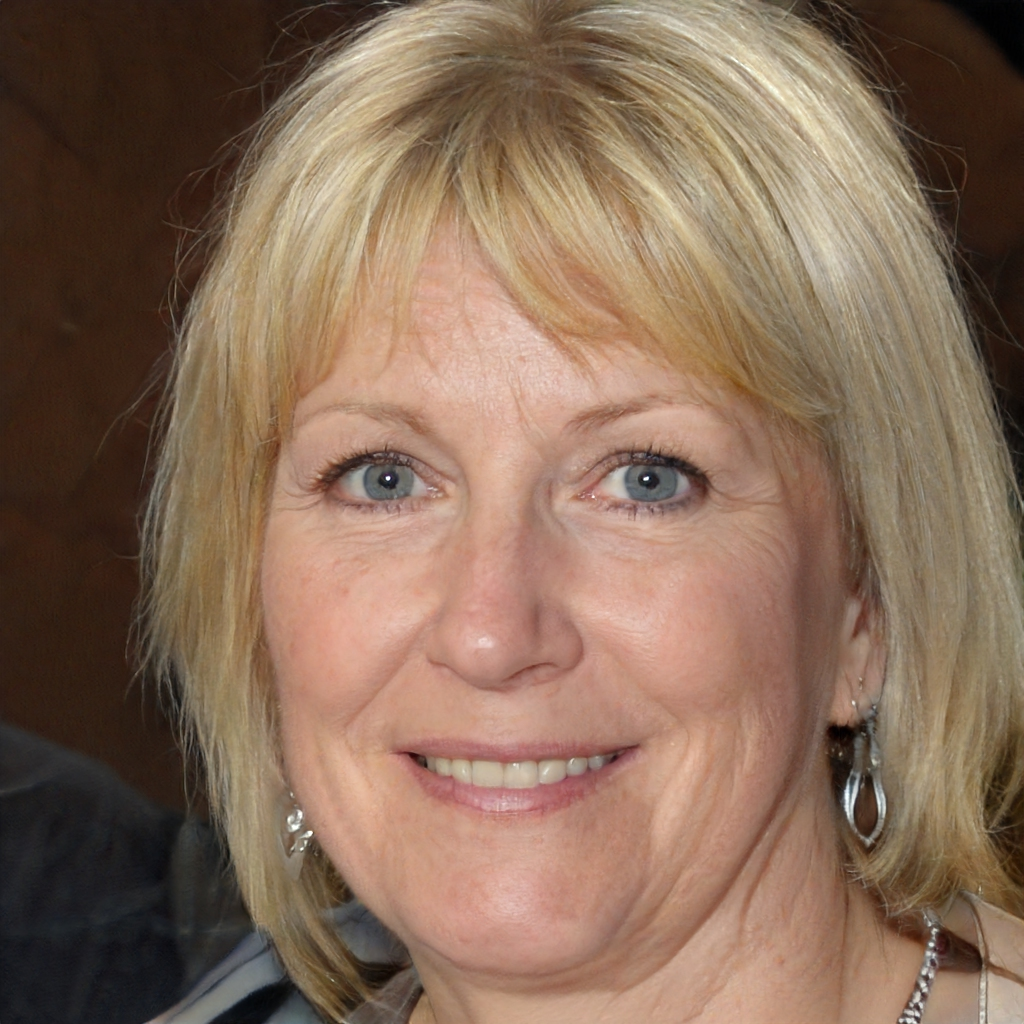
\includegraphics[height=1.5cm]{immagini/FT3-new.jpg}
	& +3 [\texttt{MT2}, \texttt{MT2}, \texttt{MT2}]\\	 
	\hline 		
	\cellcolor[HTML]{b0d7ff}\texttt{PF-5}
	&\cellcolor[HTML]{e6f2ff}\texttt{MT2}
	&\vspace{.15cm}	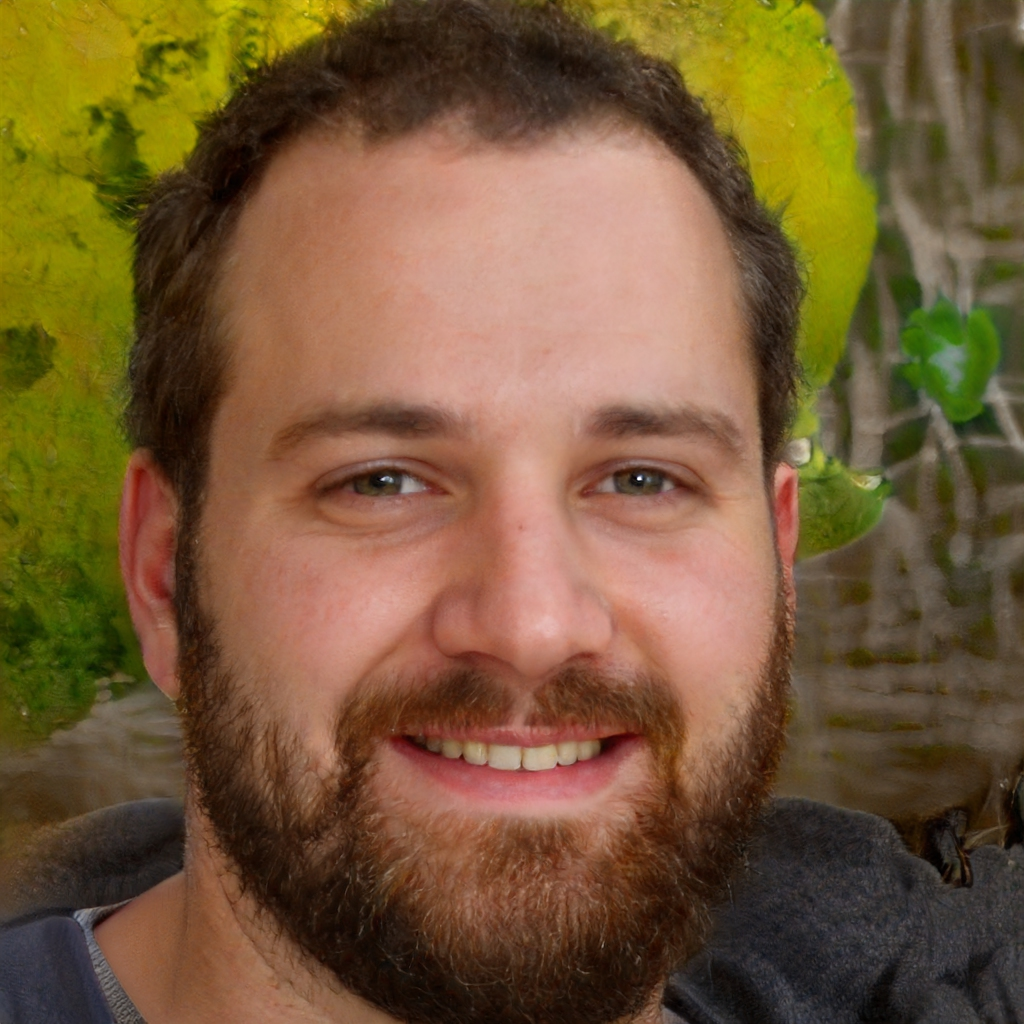
\includegraphics[height=1.5cm]{immagini/MT2.jpg}
	&\vspace{.15cm}	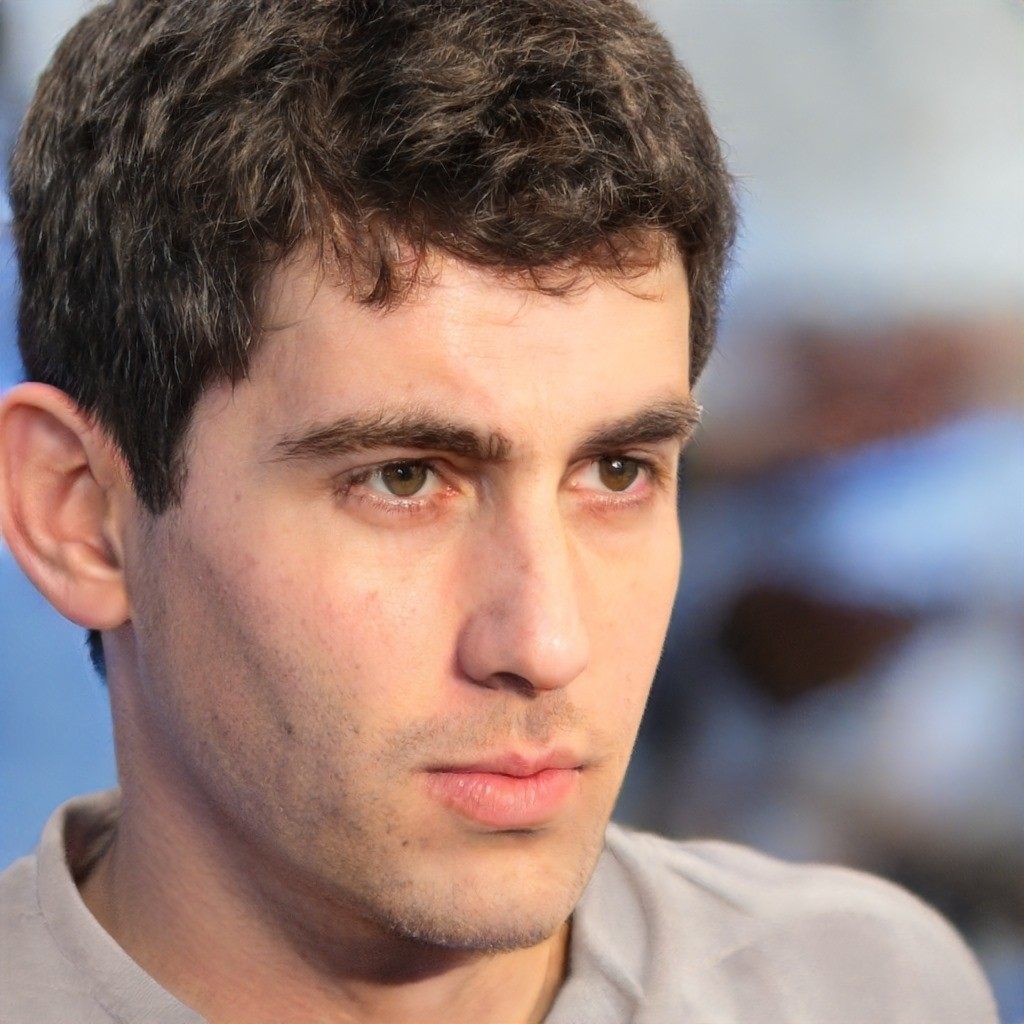
\includegraphics[height=1.5cm]{immagini/MT2-new.jpg}
	& +2 [\texttt{FT2}, \texttt{FT3}]\\	 
	\hline
	\cellcolor[HTML]{b0d7ff}\texttt{PF-3}
	&\cellcolor[HTML]{e6f2ff}\texttt{MT3}
	&\vspace{.15cm}	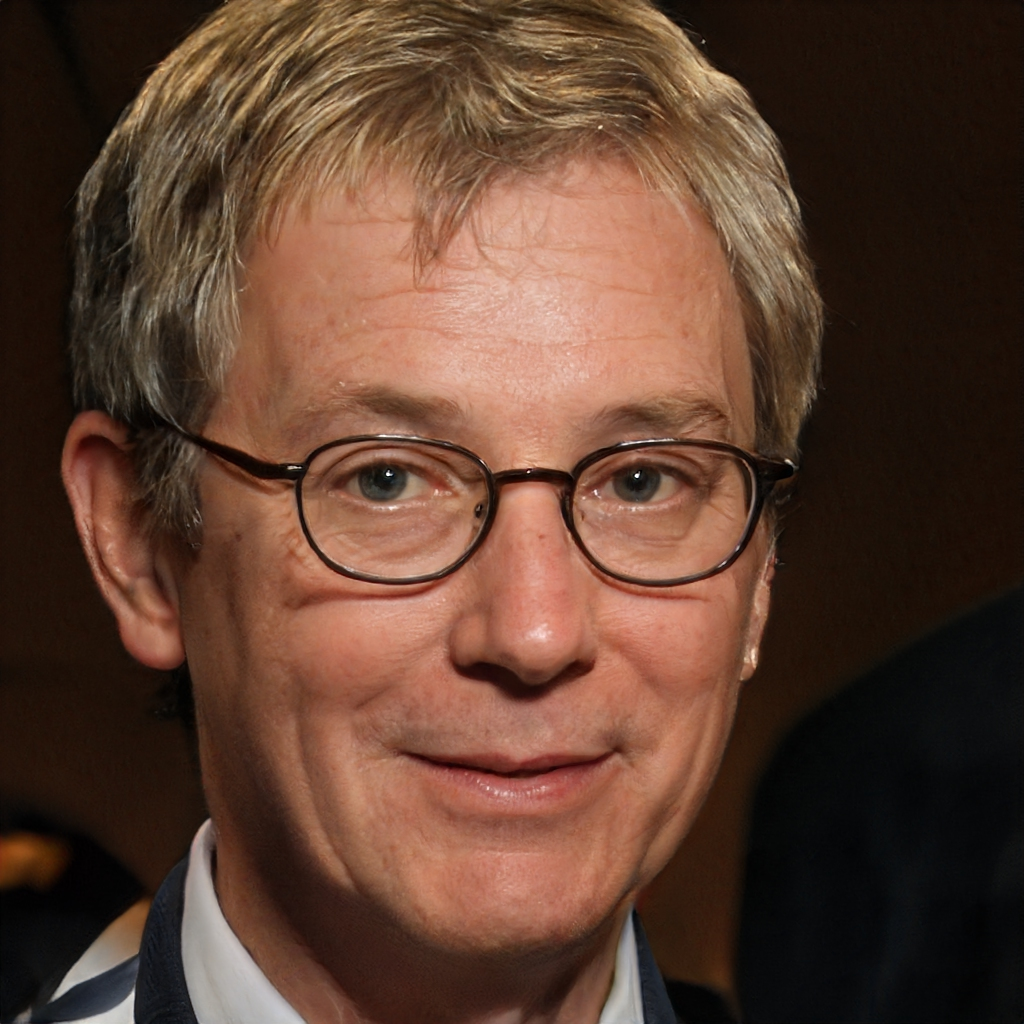
\includegraphics[height=1.5cm]{immagini/MT3.jpg}
	&\vspace{.15cm}	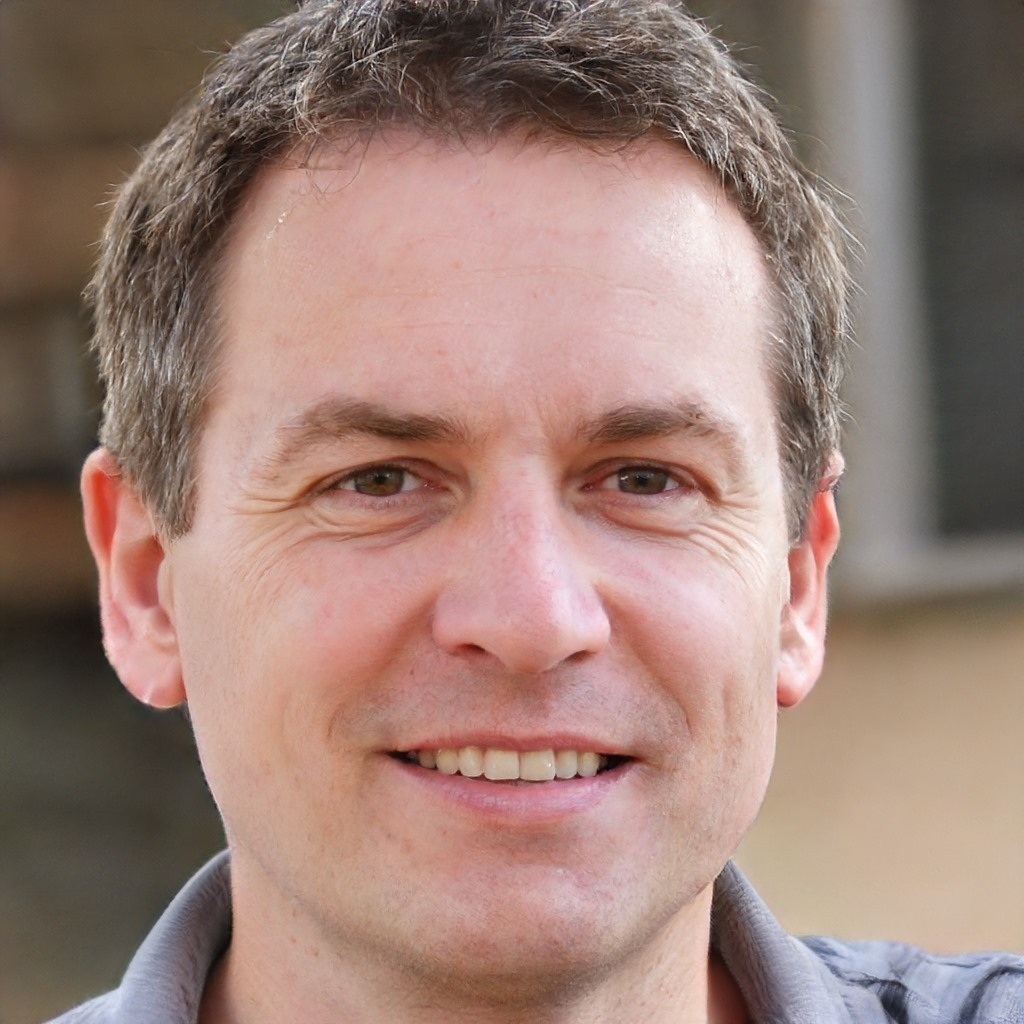
\includegraphics[height=1.5cm]{immagini/MT3-new.jpg}
	& +0 \\	 
	\hline
	\cellcolor[HTML]{b0d7ff}\texttt{PF-0}
	&\cellcolor[HTML]{e6f2ff}\texttt{MT4}
	&\vspace{.15cm}	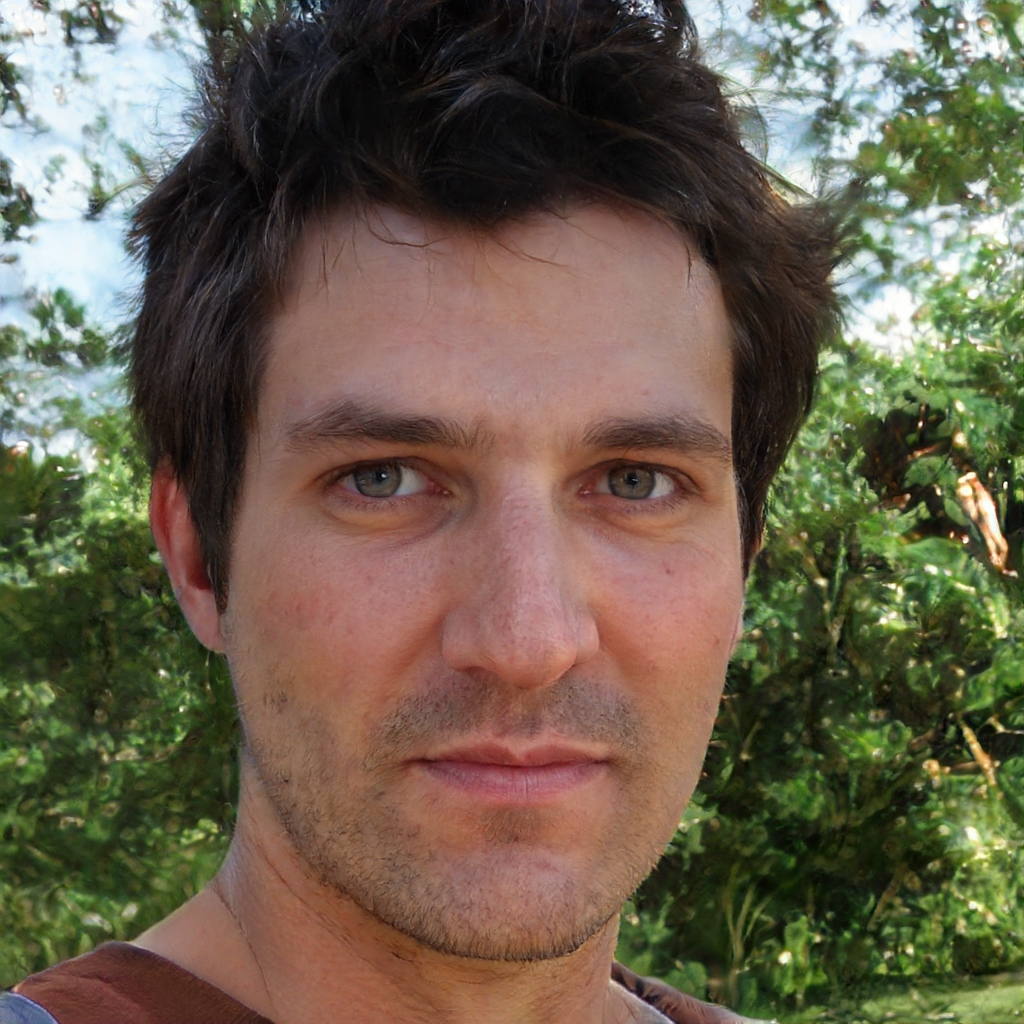
\includegraphics[height=1.5cm]{immagini/MT4.jpg}
	&\vspace{.15cm}	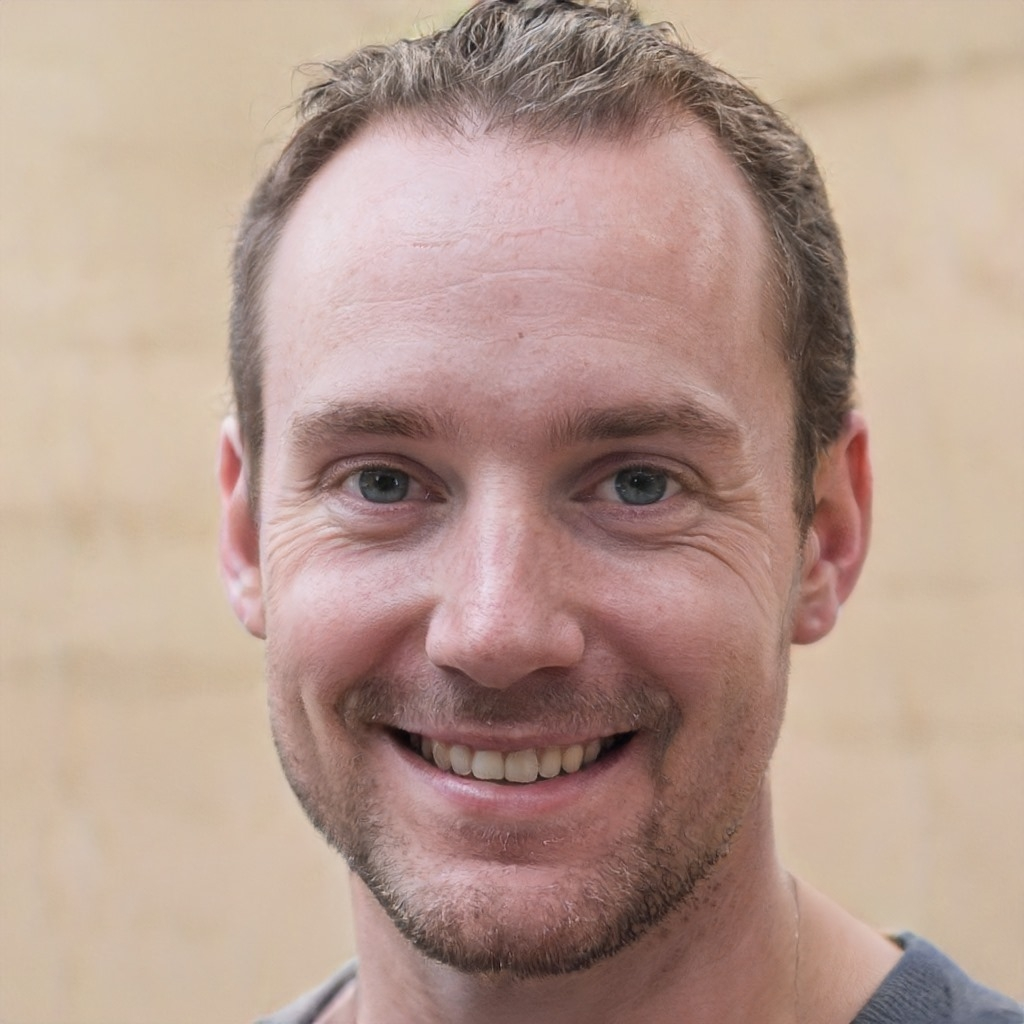
\includegraphics[height=1.5cm]{immagini/MT4-new.jpg}
	&+2 = [\texttt{FF3}, \texttt{FT3}]\\
	\hline 	 	 	 	 	
\end{tabular}
\end{center}
\caption{Profiles that have changed their profile picture and related changes in accepted friend requests.}
\label{table:change-profile-pic}
\end{table}
\subsection{Unexpected situations}
\subsubsection*{Friend requests from an external profile to an attacker profile}
This is the most unexpected situation: the attacker profiles must only send the friend request. In a sense, one could say that they would have to work in the shadows. However, some attacker profiles found themselves struggling with friend requests from other real profiles! It was decided to accept all friend requests to see the behavior that these profiles would then assume, but there is nothing relevant to report, except that some profiles have started sending many messages to these attacker profiles (details in the next chapter). Attackers who have received friend requests are reported to be: \texttt{PF-0}, \texttt{PF-6}, \texttt{PF-7}, \texttt{PF-8}, \texttt{PF-9}, and \texttt{PF-11}. In particular, the \texttt{PF-6} and \texttt{PF-11} profiles have really received many requests for friendship: analyzing them both are profiles of women, both have the real profile image and are young. The papers said that friend requests from women are more easily acceptable, but even that these profiles received so many requests, well, it was not imaginable!
\subsubsection*{Victim profiles wrote messages to (female) attacker profiles, but not with so good intentions}
Facebook is a platform where people can meet and start a conversation. Well, it was assumed that some victim profiles could accept the friendship and then write messages, to understand if they really know each other in reality or even just to make new acquaintances. The thing that was not at all expected was the number of messages received. The profiles of the attackers who received messages are all women involved in this project: \texttt{PF-6}, \texttt{PF-7}, \texttt{PF-8}, \texttt{PF-9}, \texttt{PF-10}, \texttt{PF-11}. Those who have received the most messages are \texttt{PF-6}, \texttt{PF-9}, \texttt{PF-11}. All these profiles received many messages only and exclusively from men. Many of these continued to write insistently even though they received no response. The Figures \ref{fig:message-PF-9}, \ref{fig:message-PF-10} and \ref{fig:message-PF-11} show some messages received from profiles of real people who have tried to contact the attacker profiles.
\begin{figure}[H]
	\centering
	\caption{An example of a message that \texttt{PF-9} received.}
	\label{fig:message-PF-9}
	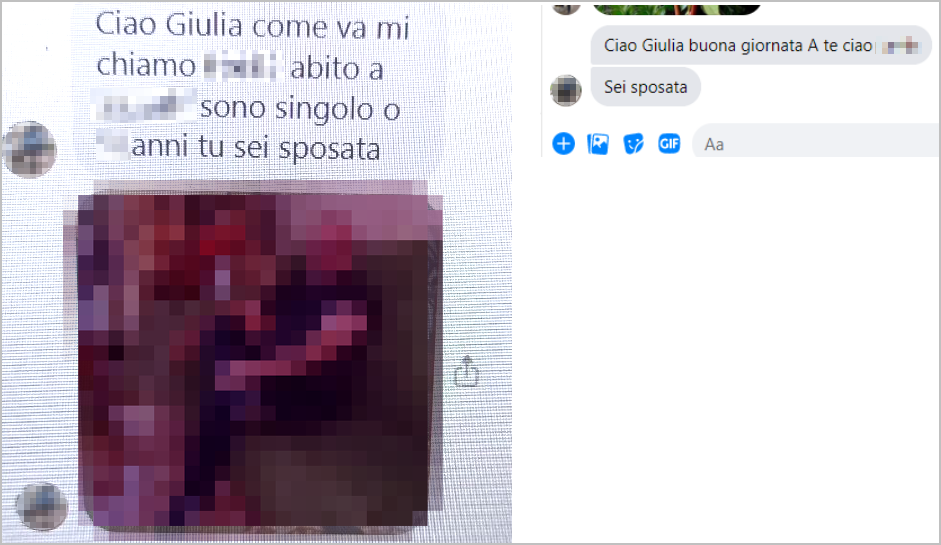
\includegraphics[height=5cm]{immagini/pf-9.png} 
\end{figure}
\begin{figure}[H]
	\centering
	\caption{An example of a message that \texttt{PF-10} received.}
	\label{fig:message-PF-10}
	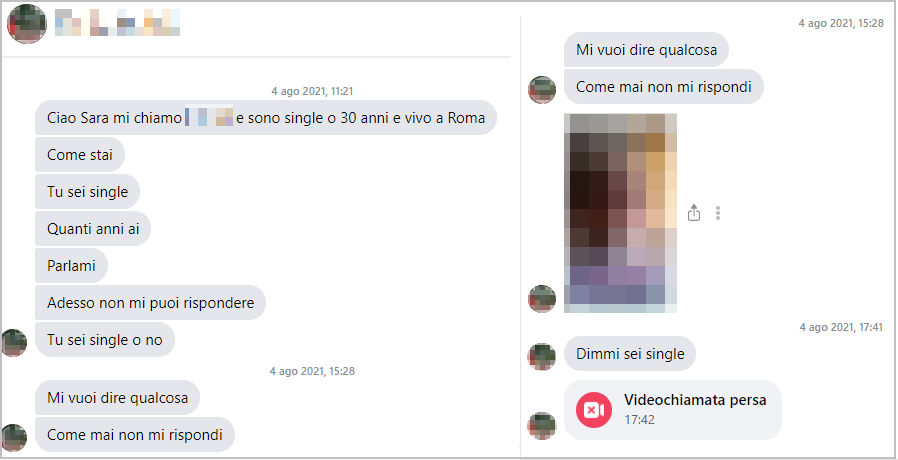
\includegraphics[height=5cm]{immagini/pf-10.png} 
\end{figure}
\begin{figure}[H]
\centering
	\caption{An example of a message that \texttt{PF-11} received.}
	\label{fig:message-PF-11}
	
\includegraphics[height=5cm]{immagini/pf-11.png} 
\end{figure}
\subsubsection*{A profile removed an attacker profile from friends}
\label{cap:discuss-removed-friends}
In short, a ``\texttt{MT3}'' victim profile removed the ``\texttt{PF-8}'' attacker profile from his friends list a few days after accepting his friend request. This situation was unexpected in the first place, but, thinking about it, it is not so strange. As some papers said, there are some people that check very carefully the person who sent them the friend request: sometimes, first, they check the profile to decide if accept the friend request; other times, first they accept the friend request and then check the profile, in order to remove it from the friends if there are some characteristics that the person doesn't like. Probably the profile more empty than usual (it is a fake profile where not a lot of content has been shared) and with a not real profile picture, made the victim suspicious, so much so as to remove this profile from the friend's list.

%********************************************************************************%
\newpage
\section{Analysis of friend requests}
\label{cap:friend-request-sent}
Each attacker profile sent 3 friend requests for each victim profile type outlined. In total, therefore, each attacker profile sent 36 friend requests. The Table \ref{table:acceptance-attacker} describes the results of the friend requests sent for each attacker profile to each type of victim profile, showing for each of them how many requests have been accepted, that could be \texttt{0/3}, \texttt{1/3}, \texttt{2/3} and \texttt{3/3}.
\par \noindent In the Chapter \ref{cap:acceptance-ranking} these results are then analyzed in more detail.

\begin{table}[H]
	\begin{center}
		\begin{tabular}[c]{ |c|c|c|c|} 
			\hline
			\cellcolor[HTML]{b0d7ff}\textsc{cod} & 
			\cellcolor[HTML]{b0d7ff}\textsc{label}& 
			\cellcolor[HTML]{b0d7ff}\textsc{victims who accepted the friend request}&		
			\cellcolor[HTML]{b0d7ff}\textsc{total}\\
			%\cellcolor[HTML]{e6f2ff}
			\hline 
%------------------------- PF-0 -----------------%
\multirow{3}{*}{\textbf{PF-0}} & \multirow{3}{*}{\texttt{MT4}}
&   \texttt{FF2: 0/3}  |  \texttt{FT2: 1/3}  |  \texttt{MF2: 2/3}  |  \texttt{MT2: 0/3} & \multirow{3}{*}{\texttt{15/36}} \\
& & \texttt{FF3: 2/3}  |  \texttt{FT3: 1/3}  |  \texttt{MF3: 1/3}  |  \texttt{MT3: 2/3} & \\
& & \texttt{FF4: 0/3}  |  \texttt{FT4: 2/3}  |  \texttt{MF4: 2/3}  |  \texttt{MT4: 2/3} & \\
\hline
%------------------------- PF-1 -----------------%
\multirow{3}{*}{\textbf{PF-1}} & \multirow{3}{*}{\texttt{MF4}}
&   \texttt{FF2: 0/3}  |  \texttt{FT2: 0/3}  |  \texttt{MF2: 1/3}  |  \texttt{MT2: 1/3} & \multirow{3}{*}{\texttt{7/36}} \\
& & \texttt{FF3: 0/3}  |  \texttt{FT3: 1/3}  |  \texttt{MF3: 0/3}  |  \texttt{MT3: 1/3} & \\
& & \texttt{FF4: 0/3}  |  \texttt{FT4: 1/3}  |  \texttt{MF4: 1/3}  |  \texttt{MT4: 1/3} & \\
\hline
%------------------------- PF-2 -----------------%
\multirow{3}{*}{\textbf{PF-2}} & \multirow{3}{*}{\texttt{MF2}}
&   \texttt{FF2: 1/3}  |  \texttt{FT2: 0/3}  |  \texttt{MF2: 0/3}  |  \texttt{MT2: 1/3} & \multirow{3}{*}{\texttt{6/36}} \\
& & \texttt{FF3: 0/3}  |  \texttt{FT3: 0/3}  |  \texttt{MF3: 2/3}  |  \texttt{MT3: 1/3} & \\
& & \texttt{FF4: 0/3}  |  \texttt{FT4: 0/3}  |  \texttt{MF4: 0/3}  |  \texttt{MT4: 1/3} & \\
\hline

%------------------------- PF-3 -----------------%
\multirow{3}{*}{\textbf{PF-3}} & \multirow{3}{*}{\texttt{MT3}}
&   \texttt{FF2: 0/3}  |  \texttt{FT2: 0/3}  |  \texttt{MF2: 0/3}  |  \texttt{MT2: 1/3} & \multirow{3}{*}{\texttt{7/36}} \\
& & \texttt{FF3: 1/3}  |  \texttt{FT3: 2/3}  |  \texttt{MF3: 1/3}  |  \texttt{MT3: 1/3} & \\
& & \texttt{FF4: 0/3}  |  \texttt{FT4: 0/3}  |  \texttt{MF4: 0/3}  |  \texttt{MT4: 1/3} & \\
\hline
%------------------------- PF-4 -----------------%
\multirow{3}{*}{\textbf{PF-4}} & \multirow{3}{*}{\texttt{MF3}}
&   \texttt{FF2: 0/3}  |  \texttt{FT2: 0/3}  |  \texttt{MF2: 0/3}  |  \texttt{MT2: 0/3} & \multirow{3}{*}{\texttt{2/36}} \\
& & \texttt{FF3: 0/3}  |  \texttt{FT3: 0/3}  |  \texttt{MF3: 0/3}  |  \texttt{MT3: 1/3} & \\
& & \texttt{FF4: 0/3}  |  \texttt{FT4: 0/3}  |  \texttt{MF4: 1/3}  |  \texttt{MT4: 0/3} & \\
\hline
%------------------------- PF-5 -----------------%
\multirow{3}{*}{\textbf{PF-5}} & \multirow{3}{*}{\texttt{MT2}}
&   \texttt{FF2: 0/3}  |  \texttt{FT2: 1/3}  |  \texttt{MF2: 1/3}  |  \texttt{MT2: 3/3} & \multirow{3}{*}{\texttt{12/36}} \\
& & \texttt{FF3: 0/3}  |  \texttt{FT3: 1/3}  |  \texttt{MF3: 1/3}  |  \texttt{MT3: 2/3} & \\
& & \texttt{FF4: 0/3}  |  \texttt{FT4: 0/3}  |  \texttt{MF4: 1/3}  |  \texttt{MT4: 2/3} & \\
\hline

%------------------------- PF-6 -----------------%
\multirow{3}{*}{\textbf{PF-6}} & \multirow{3}{*}{\texttt{FT4}}
&   \texttt{FF2: 2/3}  |  \texttt{FT2: 1/3}  |  \texttt{MF2: 1/3}  |  \texttt{MT2: 3/3} & \multirow{3}{*}{\texttt{18/36}} \\
& & \texttt{FF3: 0/3}  |  \texttt{FT3: 2/3}  |  \texttt{MF3: 0/3}  |  \texttt{MT3: 2/3} & \\
& & \texttt{FF4: 0/3}  |  \texttt{FT4: 2/3}  |  \texttt{MF4: 3/3}  |  \texttt{MT4: 2/3} & \\
\hline
%------------------------- PF-7 -----------------%
\multirow{3}{*}{\textbf{PF-7}} & \multirow{3}{*}{\texttt{FF4}}
&   \texttt{FF2: 0/3}  |  \texttt{FT2: 0/3}  |  \texttt{MF2: 0/3}  |  \texttt{MT2: 0/3} & \multirow{3}{*}{\texttt{5/36}} \\
& & \texttt{FF3: 0/3}  |  \texttt{FT3: 1/3}  |  \texttt{MF3: 0/3}  |  \texttt{MT3: 2/3} & \\
& & \texttt{FF4: 0/3}  |  \texttt{FT4: 0/3}  |  \texttt{MF4: 1/3}  |  \texttt{MT4: 1/3} & \\
\hline
%------------------------- PF-8 -----------------%
\multirow{3}{*}{\textbf{PF-8}} & \multirow{3}{*}{\texttt{FF2}}
&   \texttt{FF2: 1/3}  |  \texttt{FT2: 0/3}  |  \texttt{MF2: 1/3}  |  \texttt{MT2: 1/3} & \multirow{3}{*}{\texttt{9/36}} \\
& & \texttt{FF3: 0/3}  |  \texttt{FT3: 0/3}  |  \texttt{MF3: 2/3}  |  \texttt{MT3: 2/3} & \\
& & \texttt{FF4: 0/3}  |  \texttt{FT4: 0/3}  |  \texttt{MF4: 1/3}  |  \texttt{MT4: 3/3} & \\
\hline

%------------------------- PF-9 -----------------%
\multirow{3}{*}{\textbf{PF-9}} & \multirow{3}{*}{\texttt{FT3}}
&   \texttt{FF2: 0/3}  |  \texttt{FT2: 0/3}  |  \texttt{MF2: 0/3}  |  \texttt{MT2: 2/3} & \multirow{3}{*}{\texttt{10/36}} \\
& & \texttt{FF3: 1/3}  |  \texttt{FT3: 0/3}  |  \texttt{MF3: 2/3}  |  \texttt{MT3: 2/3} & \\
& & \texttt{FF4: 0/3}  |  \texttt{FT4: 1/3}  |  \texttt{MF4: 0/3}  |  \texttt{MT4: 1/3} & \\
\hline
%------------------------- PF-10 -----------------%
\multirow{3}{*}{\textbf{PF-10}} & \multirow{3}{*}{\texttt{FF3}}
&   \texttt{FF2: 0/3}  |  \texttt{FT2: 1/3}  |  \texttt{MF2: 0/3}  |  \texttt{MT2: 0/3} & \multirow{3}{*}{\texttt{7/36}} \\
& & \texttt{FF3: 1/3}  |  \texttt{FT3: 0/3}  |  \texttt{MF3: 0/3}  |  \texttt{MT3: 1/3} & \\
& & \texttt{FF4: 0/3}  |  \texttt{FT4: 1/3}  |  \texttt{MF4: 1/3}  |  \texttt{MT4: 2/3} & \\
\hline
%------------------------- PF-11 -----------------%
\multirow{3}{*}{\textbf{PF-11}} & \multirow{3}{*}{\texttt{FT2}}
&   \texttt{FF2: 0/3}  |  \texttt{FT2: 1/3}  |  \texttt{MF2: 1/3}  |  \texttt{MT2: 2/3} & \multirow{3}{*}{\texttt{16/36}} \\
& & \texttt{FF3: 2/3}  |  \texttt{FT3: 1/3}  |  \texttt{MF3: 2/3}  |  \texttt{MT3: 2/3} & \\
& & \texttt{FF4: 1/3}  |  \texttt{FT4: 1/3}  |  \texttt{MF4: 2/3}  |  \texttt{MT4: 1/3} & \\
\hline			
		\end{tabular}
	\end{center}
	\caption{Table that shows the results of friend requests sent from each attacker profile.}
	\label{table:acceptance-attacker}
\end{table}

\subsection{Friend requests acceptance analysis during the time}
With the \texttt{get-distribution.py} tool (Chapter \ref{cap:distribution-update}) it has been possible to trace over time how the various types of victims have accepted requests for friendship.
\par \noindent 
This first analysis of the data collected wants to grasp the difference in people's acceptance of friend requests: some people tend not to immediately accept the friend request they receive or, on the contrary, do not wait and accept the request without thinking much. So this first analysis wants to show which are the profiles that accept friend requests more easily and, vice versa, what are the types of profiles that are unlikely to accept an unknown friend request.
\par \noindent 
It was decided to compare the results of the analysis carried out a couple of weeks after sending the friend requests (30th July) with the results from the last analysis carried out (6th September). Showing the results from the data collected before 30th July would not be very interesting because the time passed is too little and the information would be mostly incomplete.
\par \noindent 
In the Table \ref{table:female-accept} reports the collected data on the profiles victim women, while in the Table \ref{table:male-accept} shows the data collected regarding the profiles victim men: in both tables for each victim profile there are two columns, the first one, which has a light grey background, shows the data collected for that specific victim with the attacker profile on 30th July, and the second column which has a dark grey background shows the data collected on 6th September.
\par \noindent 
Comparing the two tables, it can be seen that \textit{men accept friend requests in less time than women}: already on 30th July, 20 men had accepted friend requests only against 11 women. This is because, unlike men, women leave friend requests pending longer, probably to better understand the person they are dealing with.
\par \noindent 
Furthermore, it can be seen that \textit{men accept friend requests more easily than women}: even at the end of the analysis period, so on 6th September, men accepted more friend requests (58 in total) than women (35 in total).
Probably, this is because women are more suspicious and pay more attention to the profiles that sent the friend request than men.
\par \noindent 
A very interesting result is that \textit{profiles that have a real profile picture accept friend requests more easily} and, on the other hand, \textit{profiles that have a non-real profile picture accept more hardly friend requests}. 
On 30th July, only 6 profiles with the non-real profile image had accepted the friendship out of 31 total, so 25 profiles with the real profile image accepted the friend request immediately, about 80\%.
In the same way, on 6th September, the profiles with the real profile image that accepted the friend request were 72 out of 113 total friend requests accepted, that is about 64\%.
This is probably because a person with a real profile photo is more confident and exposes himself with more confidence also because she has more confidence in the social platform where she publishes her data and therefore does not think too much and accepts friend requests more easily. So, if a person puts the profile picture not real, it is probably to hide or protect themselves and for this reason, it is more difficult for this profile to accept friend requests.
\par \noindent 
Crossing these results, it can be stated that the profiles that generally accept friend requests more easily are the profiles of men with the real profile picture.
\newpage
\begin{table}[H]
	\centering
	\caption{How female victims accept friend requests during the time. \\ (Light grey background columns show data collected on 30th July, dark grey background columns show data collected on 6th September).}
	\label{table:female-accept}
	\begin{tabular}[c]{ |c|c|c|c|c|c|c|c|c|c|c|c|c| } 
		\hline
		\backslashbox{\phantom{"}}{\phantom{"}} &  			
		\multicolumn{2}{|c|}{\cellcolor[HTML]{FFFFFF}\texttt{FF2}} & 
		\multicolumn{2}{|c|}{\cellcolor[HTML]{FFFFFF}\texttt{FF3}} &
		\multicolumn{2}{|c|}{\cellcolor[HTML]{FFFFFF}\texttt{FF4}} & 
		\multicolumn{2}{|c|}{\cellcolor[HTML]{FFFFFF}\texttt{FT2}} & 
		\multicolumn{2}{|c|}{\cellcolor[HTML]{FFFFFF}\texttt{FT3}} &
		\multicolumn{2}{|c|}{\cellcolor[HTML]{FFFFFF}\texttt{FT4}} \\
		%
		\hline 
		\cellcolor[HTML]{FFFFFF}\texttt{PF-0} & 
		\cellcolor[HTML]{F5F5F5}\texttt{--} & \cellcolor[HTML]{D3D3D3}\texttt{--} &
		\cellcolor[HTML]{F5F5F5}\texttt{--} & \cellcolor[HTML]{D3D3D3}\texttt{2} &
		\cellcolor[HTML]{F5F5F5}\texttt{--} & \cellcolor[HTML]{D3D3D3}\texttt{--} & 
		\cellcolor[HTML]{F5F5F5}\texttt{--} & \cellcolor[HTML]{D3D3D3}\texttt{1} &
		\cellcolor[HTML]{F5F5F5}\texttt{--} & \cellcolor[HTML]{D3D3D3}\texttt{1} &
		\cellcolor[HTML]{F5F5F5}\texttt{1} & \cellcolor[HTML]{D3D3D3}\texttt{2} \\
		\hline
		\cellcolor[HTML]{FFFFFF}\texttt{PF-1} & 
		\cellcolor[HTML]{F5F5F5}\texttt{--} & \cellcolor[HTML]{D3D3D3}\texttt{--} &
		\cellcolor[HTML]{F5F5F5}\texttt{--} & \cellcolor[HTML]{D3D3D3}\texttt{--} &
		\cellcolor[HTML]{F5F5F5}\texttt{--} & \cellcolor[HTML]{D3D3D3}\texttt{--} & 
		\cellcolor[HTML]{F5F5F5}\texttt{--} & \cellcolor[HTML]{D3D3D3}\texttt{--} &
		\cellcolor[HTML]{F5F5F5}\texttt{--} & \cellcolor[HTML]{D3D3D3}\texttt{1} &
		\cellcolor[HTML]{F5F5F5}\texttt{1} & \cellcolor[HTML]{D3D3D3}\texttt{1} \\
		\hline 
		\cellcolor[HTML]{FFFFFF}\texttt{PF-2} & 
		\cellcolor[HTML]{F5F5F5}\texttt{1} & \cellcolor[HTML]{D3D3D3}\texttt{1} &
		\cellcolor[HTML]{F5F5F5}\texttt{--} & \cellcolor[HTML]{D3D3D3}\texttt{--} &
		\cellcolor[HTML]{F5F5F5}\texttt{--} & \cellcolor[HTML]{D3D3D3}\texttt{--} & 
		\cellcolor[HTML]{F5F5F5}\texttt{--} & \cellcolor[HTML]{D3D3D3}\texttt{--} &
		\cellcolor[HTML]{F5F5F5}\texttt{--} & \cellcolor[HTML]{D3D3D3}\texttt{--} &
		\cellcolor[HTML]{F5F5F5}\texttt{--} & \cellcolor[HTML]{D3D3D3}\texttt{--} \\
		\hline 
		\cellcolor[HTML]{FFFFFF}\texttt{PF-3} & 
		\cellcolor[HTML]{F5F5F5}\texttt{--} & \cellcolor[HTML]{D3D3D3}\texttt{--} &
		\cellcolor[HTML]{F5F5F5}\texttt{--} & \cellcolor[HTML]{D3D3D3}\texttt{1} &
		\cellcolor[HTML]{F5F5F5}\texttt{--} & \cellcolor[HTML]{D3D3D3}\texttt{--} & 
		\cellcolor[HTML]{F5F5F5}\texttt{--} & \cellcolor[HTML]{D3D3D3}\texttt{--} &
		\cellcolor[HTML]{F5F5F5}\texttt{--} & \cellcolor[HTML]{D3D3D3}\texttt{2} &
		\cellcolor[HTML]{F5F5F5}\texttt{--} & \cellcolor[HTML]{D3D3D3}\texttt{--} \\
		\hline 
		\cellcolor[HTML]{FFFFFF}\texttt{PF-4} & 
		\cellcolor[HTML]{F5F5F5}\texttt{--} & \cellcolor[HTML]{D3D3D3}\texttt{--} &
		\cellcolor[HTML]{F5F5F5}\texttt{--} & \cellcolor[HTML]{D3D3D3}\texttt{--} &
		\cellcolor[HTML]{F5F5F5}\texttt{--} & \cellcolor[HTML]{D3D3D3}\texttt{--} & 
		\cellcolor[HTML]{F5F5F5}\texttt{--} & \cellcolor[HTML]{D3D3D3}\texttt{--} &
		\cellcolor[HTML]{F5F5F5}\texttt{--} & \cellcolor[HTML]{D3D3D3}\texttt{--} &
		\cellcolor[HTML]{F5F5F5}\texttt{--} & \cellcolor[HTML]{D3D3D3}\texttt{--} \\
		\hline 
		\cellcolor[HTML]{FFFFFF}\texttt{PF-5} & 
		\cellcolor[HTML]{F5F5F5}\texttt{--} & \cellcolor[HTML]{D3D3D3}\texttt{--} &
		\cellcolor[HTML]{F5F5F5}\texttt{--} & \cellcolor[HTML]{D3D3D3}\texttt{--} &
		\cellcolor[HTML]{F5F5F5}\texttt{--} & \cellcolor[HTML]{D3D3D3}\texttt{--} & 
		\cellcolor[HTML]{F5F5F5}\texttt{--} & \cellcolor[HTML]{D3D3D3}\texttt{1} &
		\cellcolor[HTML]{F5F5F5}\texttt{--} & \cellcolor[HTML]{D3D3D3}\texttt{1} &
		\cellcolor[HTML]{F5F5F5}\texttt{--} & \cellcolor[HTML]{D3D3D3}\texttt{--} \\
		\hline 
		\cellcolor[HTML]{FFFFFF}\texttt{PF-6} & 
		\cellcolor[HTML]{F5F5F5}\texttt{1} & \cellcolor[HTML]{D3D3D3}\texttt{2} &
		\cellcolor[HTML]{F5F5F5}\texttt{--} & \cellcolor[HTML]{D3D3D3}\texttt{--} &
		\cellcolor[HTML]{F5F5F5}\texttt{--} & \cellcolor[HTML]{D3D3D3}\texttt{--} & 
		\cellcolor[HTML]{F5F5F5}\texttt{--} & \cellcolor[HTML]{D3D3D3}\texttt{1} &
		\cellcolor[HTML]{F5F5F5}\texttt{1} & \cellcolor[HTML]{D3D3D3}\texttt{2} &
		\cellcolor[HTML]{F5F5F5}\texttt{1} & \cellcolor[HTML]{D3D3D3}\texttt{2} \\
		\hline 
		\cellcolor[HTML]{FFFFFF}\texttt{PF-7} & 
		\cellcolor[HTML]{F5F5F5}\texttt{--} & \cellcolor[HTML]{D3D3D3}\texttt{--} &
		\cellcolor[HTML]{F5F5F5}\texttt{--} & \cellcolor[HTML]{D3D3D3}\texttt{--} &
		\cellcolor[HTML]{F5F5F5}\texttt{--} & \cellcolor[HTML]{D3D3D3}\texttt{--} & 
		\cellcolor[HTML]{F5F5F5}\texttt{--} & \cellcolor[HTML]{D3D3D3}\texttt{--} &
		\cellcolor[HTML]{F5F5F5}\texttt{1} & \cellcolor[HTML]{D3D3D3}\texttt{1} &
		\cellcolor[HTML]{F5F5F5}\texttt{--} & \cellcolor[HTML]{D3D3D3}\texttt{--} \\
		\hline 
		\cellcolor[HTML]{FFFFFF}\texttt{PF-8} & 
		\cellcolor[HTML]{F5F5F5}\texttt{1} & \cellcolor[HTML]{D3D3D3}\texttt{1} &
		\cellcolor[HTML]{F5F5F5}\texttt{--} & \cellcolor[HTML]{D3D3D3}\texttt{--} &
		\cellcolor[HTML]{F5F5F5}\texttt{--} & \cellcolor[HTML]{D3D3D3}\texttt{--} & 
		\cellcolor[HTML]{F5F5F5}\texttt{--} & \cellcolor[HTML]{D3D3D3}\texttt{--} &
		\cellcolor[HTML]{F5F5F5}\texttt{--} & \cellcolor[HTML]{D3D3D3}\texttt{--} &
		\cellcolor[HTML]{F5F5F5}\texttt{--} & \cellcolor[HTML]{D3D3D3}\texttt{--} \\
		\hline 
		\cellcolor[HTML]{FFFFFF}\texttt{PF-9} & 
		\cellcolor[HTML]{F5F5F5}\texttt{--} & \cellcolor[HTML]{D3D3D3}\texttt{1} &
		\cellcolor[HTML]{F5F5F5}\texttt{--} & \cellcolor[HTML]{D3D3D3}\texttt{--} &
		\cellcolor[HTML]{F5F5F5}\texttt{--} & \cellcolor[HTML]{D3D3D3}\texttt{1} & 
		\cellcolor[HTML]{F5F5F5}\texttt{--} & \cellcolor[HTML]{D3D3D3}\texttt{--} &
		\cellcolor[HTML]{F5F5F5}\texttt{--} & \cellcolor[HTML]{D3D3D3}\texttt{--} &
		\cellcolor[HTML]{F5F5F5}\texttt{1} & \cellcolor[HTML]{D3D3D3}\texttt{1} \\
		\hline 
		\cellcolor[HTML]{FFFFFF}\texttt{PF-10} & 
		\cellcolor[HTML]{F5F5F5}\texttt{--} & \cellcolor[HTML]{D3D3D3}\texttt{--} &
		\cellcolor[HTML]{F5F5F5}\texttt{1} & \cellcolor[HTML]{D3D3D3}\texttt{1} &
		\cellcolor[HTML]{F5F5F5}\texttt{--} & \cellcolor[HTML]{D3D3D3}\texttt{--} & 
		\cellcolor[HTML]{F5F5F5}\texttt{--} & \cellcolor[HTML]{D3D3D3}\texttt{1} &
		\cellcolor[HTML]{F5F5F5}\texttt{--} & \cellcolor[HTML]{D3D3D3}\texttt{--} &
		\cellcolor[HTML]{F5F5F5}\texttt{1} & \cellcolor[HTML]{D3D3D3}\texttt{1} \\
		\hline 
		\cellcolor[HTML]{FFFFFF}\texttt{PF-11} & 
		\cellcolor[HTML]{F5F5F5}\texttt{--} & \cellcolor[HTML]{D3D3D3}\texttt{--} &
		\cellcolor[HTML]{F5F5F5}\texttt{--} & \cellcolor[HTML]{D3D3D3}\texttt{2} &
		\cellcolor[HTML]{F5F5F5}\texttt{--} & \cellcolor[HTML]{D3D3D3}\texttt{1} & 
		\cellcolor[HTML]{F5F5F5}\texttt{--} & \cellcolor[HTML]{D3D3D3}\texttt{1} &
		\cellcolor[HTML]{F5F5F5}\texttt{--} & \cellcolor[HTML]{D3D3D3}\texttt{1} &
		\cellcolor[HTML]{F5F5F5}\texttt{--} & \cellcolor[HTML]{D3D3D3}\texttt{1} \\
		\hline 
	\end{tabular}
\end{table}
\begin{table}[H]
	\centering
	\caption{How male victims accept friend requests during the time. \\ (Light grey background columns show data collected on 30th July, dark grey background columns show data collected on 6th September).}
	\label{table:male-accept}
	\begin{tabular}[c]{ |c|c|c|c|c|c|c|c|c|c|c|c|c| } 
		\hline
		\backslashbox{\phantom{"}}{\phantom{"}} &   			
		\multicolumn{2}{|c|}{\cellcolor[HTML]{FFFFFF}\texttt{MF2}} & 
		\multicolumn{2}{|c|}{\cellcolor[HTML]{FFFFFF}\texttt{MF3}} &
		\multicolumn{2}{|c|}{\cellcolor[HTML]{FFFFFF}\texttt{MF4}} & 
		\multicolumn{2}{|c|}{\cellcolor[HTML]{FFFFFF}\texttt{MT2}} & 
		\multicolumn{2}{|c|}{\cellcolor[HTML]{FFFFFF}\texttt{MT3}} &
		\multicolumn{2}{|c|}{\cellcolor[HTML]{FFFFFF}\texttt{MT4}} \\
		%
		\hline 
		\cellcolor[HTML]{FFFFFF}\texttt{PF-0} & 
		\cellcolor[HTML]{F5F5F5}\texttt{--} & \cellcolor[HTML]{D3D3D3}\texttt{2} &
		\cellcolor[HTML]{F5F5F5}\texttt{--} & \cellcolor[HTML]{D3D3D3}\texttt{1} &
		\cellcolor[HTML]{F5F5F5}\texttt{--} & \cellcolor[HTML]{D3D3D3}\texttt{2} & 
		\cellcolor[HTML]{F5F5F5}\texttt{--} & \cellcolor[HTML]{D3D3D3}\texttt{--} &
		\cellcolor[HTML]{F5F5F5}\texttt{1} & \cellcolor[HTML]{D3D3D3}\texttt{2} &
		\cellcolor[HTML]{F5F5F5}\texttt{1} & \cellcolor[HTML]{D3D3D3}\texttt{2} \\
		\hline 
		\cellcolor[HTML]{FFFFFF}\texttt{PF-1} & 
		\cellcolor[HTML]{F5F5F5}\texttt{--} & \cellcolor[HTML]{D3D3D3}\texttt{1} &
		\cellcolor[HTML]{F5F5F5}\texttt{--} & \cellcolor[HTML]{D3D3D3}\texttt{--} &
		\cellcolor[HTML]{F5F5F5}\texttt{1} & \cellcolor[HTML]{D3D3D3}\texttt{1} & 
		\cellcolor[HTML]{F5F5F5}\texttt{1} & \cellcolor[HTML]{D3D3D3}\texttt{1} &
		\cellcolor[HTML]{F5F5F5}\texttt{1} & \cellcolor[HTML]{D3D3D3}\texttt{1} &
		\cellcolor[HTML]{F5F5F5}\texttt{--} & \cellcolor[HTML]{D3D3D3}\texttt{1} \\
		\hline 
		\cellcolor[HTML]{FFFFFF}\texttt{PF-2} & 
		\cellcolor[HTML]{F5F5F5}\texttt{--} & \cellcolor[HTML]{D3D3D3}\texttt{--} &
		\cellcolor[HTML]{F5F5F5}\texttt{--} & \cellcolor[HTML]{D3D3D3}\texttt{2} &
		\cellcolor[HTML]{F5F5F5}\texttt{--} & \cellcolor[HTML]{D3D3D3}\texttt{--} & 
		\cellcolor[HTML]{F5F5F5}\texttt{--} & \cellcolor[HTML]{D3D3D3}\texttt{1} &
		\cellcolor[HTML]{F5F5F5}\texttt{--} & \cellcolor[HTML]{D3D3D3}\texttt{1} &
		\cellcolor[HTML]{F5F5F5}\texttt{--} & \cellcolor[HTML]{D3D3D3}\texttt{1} \\
		\hline 
		\cellcolor[HTML]{FFFFFF}\texttt{PF-3} & 
		\cellcolor[HTML]{F5F5F5}\texttt{--} & \cellcolor[HTML]{D3D3D3}\texttt{--} &
		\cellcolor[HTML]{F5F5F5}\texttt{--} & \cellcolor[HTML]{D3D3D3}\texttt{1} &
		\cellcolor[HTML]{F5F5F5}\texttt{--} & \cellcolor[HTML]{D3D3D3}\texttt{--} & 
		\cellcolor[HTML]{F5F5F5}\texttt{1} & \cellcolor[HTML]{D3D3D3}\texttt{1} &
		\cellcolor[HTML]{F5F5F5}\texttt{--} & \cellcolor[HTML]{D3D3D3}\texttt{1} &
		\cellcolor[HTML]{F5F5F5}\texttt{--} & \cellcolor[HTML]{D3D3D3}\texttt{1} \\
		\hline 
		\cellcolor[HTML]{FFFFFF}\texttt{PF-4} & 
		\cellcolor[HTML]{F5F5F5}\texttt{--} & \cellcolor[HTML]{D3D3D3}\texttt{--} &
		\cellcolor[HTML]{F5F5F5}\texttt{--} & \cellcolor[HTML]{D3D3D3}\texttt{--} &
		\cellcolor[HTML]{F5F5F5}\texttt{--} & \cellcolor[HTML]{D3D3D3}\texttt{1} & 
		\cellcolor[HTML]{F5F5F5}\texttt{--} & \cellcolor[HTML]{D3D3D3}\texttt{--} &
		\cellcolor[HTML]{F5F5F5}\texttt{--} & \cellcolor[HTML]{D3D3D3}\texttt{1} &
		\cellcolor[HTML]{F5F5F5}\texttt{--} & \cellcolor[HTML]{D3D3D3}\texttt{--} \\
		\hline 
		\cellcolor[HTML]{FFFFFF}\texttt{PF-5} & 
		\cellcolor[HTML]{F5F5F5}\texttt{--} & \cellcolor[HTML]{D3D3D3}\texttt{1} &
		\cellcolor[HTML]{F5F5F5}\texttt{--} & \cellcolor[HTML]{D3D3D3}\texttt{1} &
		\cellcolor[HTML]{F5F5F5}\texttt{--} & \cellcolor[HTML]{D3D3D3}\texttt{1} & 
		\cellcolor[HTML]{F5F5F5}\texttt{3} & \cellcolor[HTML]{D3D3D3}\texttt{3} &
		\cellcolor[HTML]{F5F5F5}\texttt{1} & \cellcolor[HTML]{D3D3D3}\texttt{2} &
		\cellcolor[HTML]{F5F5F5}\texttt{--} & \cellcolor[HTML]{D3D3D3}\texttt{2} \\
		\hline 
		\cellcolor[HTML]{FFFFFF}\texttt{PF-6} & 
		\cellcolor[HTML]{F5F5F5}\texttt{--} & \cellcolor[HTML]{D3D3D3}\texttt{1} &
		\cellcolor[HTML]{F5F5F5}\texttt{--} & \cellcolor[HTML]{D3D3D3}\texttt{--} &
		\cellcolor[HTML]{F5F5F5}\texttt{--} & \cellcolor[HTML]{D3D3D3}\texttt{3} & 
		\cellcolor[HTML]{F5F5F5}\texttt{--} & \cellcolor[HTML]{D3D3D3}\texttt{3} &
		\cellcolor[HTML]{F5F5F5}\texttt{1} & \cellcolor[HTML]{D3D3D3}\texttt{2} &
		\cellcolor[HTML]{F5F5F5}\texttt{--} & \cellcolor[HTML]{D3D3D3}\texttt{2} \\
		\hline 
		\cellcolor[HTML]{FFFFFF}\texttt{PF-7} & 
		\cellcolor[HTML]{F5F5F5}\texttt{--} & \cellcolor[HTML]{D3D3D3}\texttt{--} &
		\cellcolor[HTML]{F5F5F5}\texttt{--} & \cellcolor[HTML]{D3D3D3}\texttt{--} &
		\cellcolor[HTML]{F5F5F5}\texttt{--} & \cellcolor[HTML]{D3D3D3}\texttt{1} & 
		\cellcolor[HTML]{F5F5F5}\texttt{--} & \cellcolor[HTML]{D3D3D3}\texttt{--} &
		\cellcolor[HTML]{F5F5F5}\texttt{2} & \cellcolor[HTML]{D3D3D3}\texttt{2} &
		\cellcolor[HTML]{F5F5F5}\texttt{--} & \cellcolor[HTML]{D3D3D3}\texttt{1} \\
		\hline 
		\cellcolor[HTML]{FFFFFF}\texttt{PF-8} & 
		\cellcolor[HTML]{F5F5F5}\texttt{--} & \cellcolor[HTML]{D3D3D3}\texttt{1} &
		\cellcolor[HTML]{F5F5F5}\texttt{--} & \cellcolor[HTML]{D3D3D3}\texttt{--} &
		\cellcolor[HTML]{F5F5F5}\texttt{--} & \cellcolor[HTML]{D3D3D3}\texttt{1} & 
		\cellcolor[HTML]{F5F5F5}\texttt{1} & \cellcolor[HTML]{D3D3D3}\texttt{1} &
		\cellcolor[HTML]{F5F5F5}\texttt{--} & \cellcolor[HTML]{D3D3D3}\texttt{2} &
		\cellcolor[HTML]{F5F5F5}\texttt{2} & \cellcolor[HTML]{D3D3D3}\texttt{3} \\
		\hline 
		\cellcolor[HTML]{FFFFFF}\texttt{PF-9} & 
		\cellcolor[HTML]{F5F5F5}\texttt{--} & \cellcolor[HTML]{D3D3D3}\texttt{--} &
		\cellcolor[HTML]{F5F5F5}\texttt{--} & \cellcolor[HTML]{D3D3D3}\texttt{2} &
		\cellcolor[HTML]{F5F5F5}\texttt{--} & \cellcolor[HTML]{D3D3D3}\texttt{--} & 
		\cellcolor[HTML]{F5F5F5}\texttt{--} & \cellcolor[HTML]{D3D3D3}\texttt{2} &
		\cellcolor[HTML]{F5F5F5}\texttt{1} & \cellcolor[HTML]{D3D3D3}\texttt{2} &
		\cellcolor[HTML]{F5F5F5}\texttt{--} & \cellcolor[HTML]{D3D3D3}\texttt{1} \\
		\hline 
		\cellcolor[HTML]{FFFFFF}\texttt{PF-10} & 
		\cellcolor[HTML]{F5F5F5}\texttt{--} & \cellcolor[HTML]{D3D3D3}\texttt{--} &
		\cellcolor[HTML]{F5F5F5}\texttt{--} & \cellcolor[HTML]{D3D3D3}\texttt{--} &
		\cellcolor[HTML]{F5F5F5}\texttt{1} & \cellcolor[HTML]{D3D3D3}\texttt{1} & 
		\cellcolor[HTML]{F5F5F5}\texttt{--} & \cellcolor[HTML]{D3D3D3}\texttt{--} &
		\cellcolor[HTML]{F5F5F5}\texttt{--} & \cellcolor[HTML]{D3D3D3}\texttt{1} &
		\cellcolor[HTML]{F5F5F5}\texttt{1} & \cellcolor[HTML]{D3D3D3}\texttt{2} \\
		\hline 
		\cellcolor[HTML]{FFFFFF}\texttt{PF-11} & 
		\cellcolor[HTML]{F5F5F5}\texttt{--} & \cellcolor[HTML]{D3D3D3}\texttt{1} &
		\cellcolor[HTML]{F5F5F5}\texttt{--} & \cellcolor[HTML]{D3D3D3}\texttt{2} &
		\cellcolor[HTML]{F5F5F5}\texttt{--} & \cellcolor[HTML]{D3D3D3}\texttt{2} & 
		\cellcolor[HTML]{F5F5F5}\texttt{--} & \cellcolor[HTML]{D3D3D3}\texttt{2} &
		\cellcolor[HTML]{F5F5F5}\texttt{--} & \cellcolor[HTML]{D3D3D3}\texttt{2} &
		\cellcolor[HTML]{F5F5F5}\texttt{1} & \cellcolor[HTML]{D3D3D3}\texttt{1} \\
		\hline 
	\end{tabular}
\end{table}

\newpage

\subsection{Acceptance ranking of friend requests}
\label{cap:acceptance-ranking}
With the tool \texttt{report-acceptance.py} (Chapter \ref{cap:tool-report-acc}) it has been possible to check which attacker profiles were accepted the most (and least) and from which victim profiles.
\par \noindent This section furnishes a report of the acceptance that the profiles of the attackers had towards the victim profiles, and it is given by the result of the analysis carried out on 6th September.\par \noindent  The Table \ref{table:ranking-attacker} shows the ranking of attacker profiles based on how many friend requests sent by it have been accepted. It is immediate to the eye that the \textit{female profiles are accepted more easily than male profiles}. In fact, out of a total of 114 friend requests accepted, female attacker profiles were accepted 65 times against 49 of the male attacker profiles.\par \noindent  Furthermore, both for men and women, \textit{the most accepted profiles are those with the real profile picture} (34/49 for men and 44/65 for women) to the detriment of those profiles with the profile picture not real (15/49 for men and 21/65 for women).
\begin{table}[H]
	\begin{center}
		\begin{tabular}[c]{ |c|c|c|c|c| } 
			\hline
			\cellcolor[HTML]{b0d7ff}\textsc{position} & 
			\cellcolor[HTML]{b0d7ff}\textsc{cod} & 
			\cellcolor[HTML]{b0d7ff}\textsc{label}& 
			\cellcolor[HTML]{b0d7ff}\textsc{friend requests accepted}& 
			\cellcolor[HTML]{b0d7ff}\textsc{ranking}\\
			%\cellcolor[HTML]{e6f2ff}
			\hline 
			\textbf{\textsc{1°}}
			&\texttt{PF-6}
			&\cellcolor[HTML]{e6f2ff}\texttt{FT4}
			& \texttt{18/36}
			& \texttt{50,00\%}\\	 
			\hline
			\textbf{\textsc{2°}}
			&\texttt{PF-11}
			&\cellcolor[HTML]{e6f2ff}\texttt{FT2}
			& \texttt{16/36}
			& \texttt{44,44\%}\\	 
			\hline
			\textbf{\textsc{3°}}
			&\texttt{PF-0}
			&\cellcolor[HTML]{e6f2ff}\texttt{MT4}
			& \texttt{15/36}
			& \texttt{41,67\%}\\	 
			\hline
			\textbf{\textsc{4°}}
			&\texttt{PF-5}
			&\cellcolor[HTML]{e6f2ff}\texttt{MT2}
			& \texttt{12/36}
			& \texttt{33,33\%}\\	 
			\hline
			\textbf{\textsc{5°}}
			&\texttt{PF-9}
			&\cellcolor[HTML]{e6f2ff}\texttt{FT4}
			& \texttt{10/36}
			& \texttt{27,78\%}\\	 
			\hline
			\textbf{\textsc{6°}}
			&\texttt{PF-8}
			&\cellcolor[HTML]{e6f2ff}\texttt{FT2}
			& \texttt{9/36}
			& \texttt{25,00\%}\\	 
			\hline
			
			\multirow{3}{*}{\textbf{\textsc{7°}}} 
			& \texttt{PF-1} & \cellcolor[HTML]{e6f2ff}\texttt{MF4} & \multirow{3}*{\texttt{7/36}}&\multirow{3}*{\texttt{19,44\%}}\\		
			& \texttt{PF-3} & \cellcolor[HTML]{e6f2ff}\texttt{MT3} & & \\
			& \texttt{PF-10} & \cellcolor[HTML]{e6f2ff}\texttt{FF3} & & \\
			
			\hline			
			\textbf{\textsc{8°}}
			&\texttt{PF-2}
			&\cellcolor[HTML]{e6f2ff}\texttt{MF2}
			& \texttt{6/36}
			& \texttt{16,67\%}\\	 
			\hline			
			\textbf{\textsc{9°}}
			&\texttt{PF-7}
			&\cellcolor[HTML]{e6f2ff}\texttt{FF4}
			& \texttt{5/36}
			& \texttt{13,89\%}\\	 
			\hline
			\textbf{\textsc{10°}}
			&\texttt{PF-4}
			&\cellcolor[HTML]{e6f2ff}\texttt{MF3}
			& \texttt{2/36}
			& \texttt{5,56\%}\\	 
			\hline
		\end{tabular}
	\end{center}
	\caption{Attacker profiles ranking.}
	\label{table:ranking-attacker}
\end{table}
The acceptance of each attacker profile by each type of victim profile is now analyzed in detail.
\newpage
\subsection*{PF-0}
It represents a \texttt{MT4} profile, that is a man with hidden age and that in his Facebook profile he has the profile picture that shows his face.
\par \noindent The Figure \ref{fig:accepted-from-PF0} represents the collected data referred to this profile. 
\begin{figure}[H]	
	\centering
	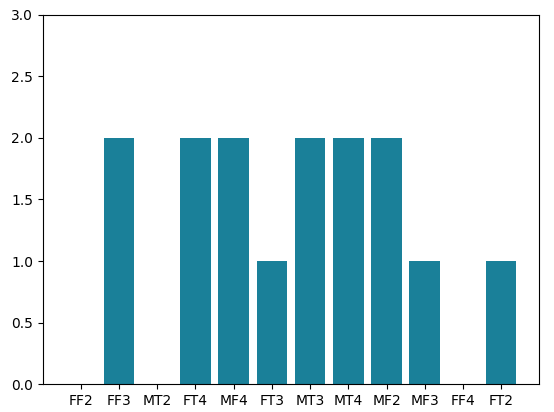
\includegraphics[height=4.5cm]{report-acceptance/PF-0.png} 
	\caption{Total of friend request accepted from \texttt{PF-0}}
	\label{fig:accepted-from-PF0}
\end{figure}
\par \noindent
In detail, it can be noted that:
\begin{enumerate} 
	\item it is more accepted from men (9) than women (6);
	\item it is accepted almost equally by both those with a real (8) and a false (7) profile picture; 
	\item it is accepted more by female profiles with the real profile picture (4) than with the false profile picture (2), unlike the male profiles who accepted this profile equally (5 had a false profile picture against 4 with a real profile picture);
	\item it is accepted more by profiles over the age of 50 (6 in total, 3 women and 3 men) and by profiles with hidden age (6 in total, 2 women and 4 men), while it is accepted only 3 times in total from profiles aged between 18 and 50 (1 woman and 2 men).
\end{enumerate}


\subsection*{PF-1}
It represents a \texttt{MF4} profile, that is a man with hidden age and that in his Facebook profile he has the profile picture where he does not show his face.
\par \noindent The Figure \ref{fig:accepted-from-PF1} represents the collected data referred to this profile. 
\begin{figure}[H]	
	\centering
	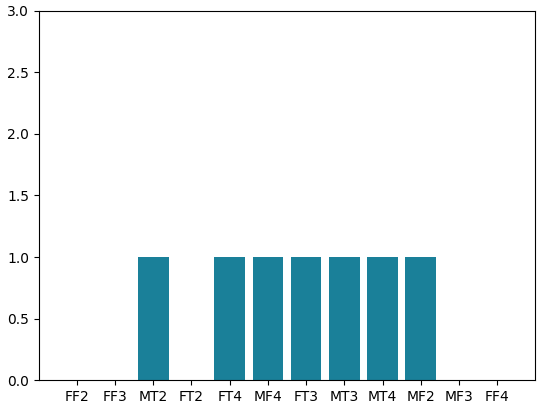
\includegraphics[height=4.5cm]{report-acceptance/PF-1.png}
	\caption{Total of friend request accepted from \texttt{PF-1}}
	\label{fig:accepted-from-PF1}
\end{figure}
\par \noindent
In detail, it can be noted that:
\begin{enumerate}
	\item it is more accepted from men (5) than women (2);
	\item it is more accepted from those profiles with a real profile picture (5) than those with a false profile picture (2); 
	\item it is accepted only by female profiles with the real profile picture (2 against 0 female profiles with false profile pictures), unlike the male profiles who accepted this profile equally (2 had a false profile picture against 3 with a real profile picture);
	\item it is accepted more by profiles with hidden age (3 in total, 1 woman and 2 men), followed by profiles over the age of 50 (2 in total, 1 woman and 1 man), while it was accepted only 2 times in total from profiles aged between 18 and 50 (0 women and 2 men).
\end{enumerate}


\subsection*{PF-2}
It represents a \texttt{MF2} profile, that is a man aged between 18 and 50 and that in his Facebook profile he has the profile picture that does not show his face.
\par \noindent The Figure \ref{fig:accepted-from-PF2} represents the collected data referred to this profile.
\begin{figure}[H]	
	\centering
	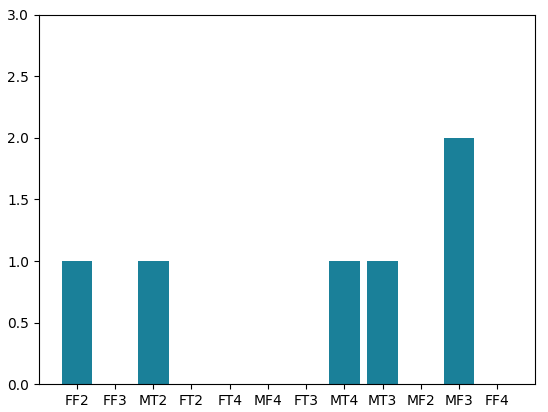
\includegraphics[height=4.5cm]{report-acceptance/PF-2.png} 
	\caption{Total of friend request accepted from \texttt{PF-2}}
	\label{fig:accepted-from-PF2}
\end{figure}
\par \noindent
In detail, it can be noted that:
\begin{enumerate} 
	\item it is more accepted from men (5) than women (1);
	\item it is accepted almost equally by both those with a real (3) and a false (3) profile picture;
	\item it is accepted only by female profiles with the false profile picture (1 against 0 female profiles with real profile pictures), unlike the male profiles who accepted this profile almost equally (2 had a false profile picture against 3 with a real profile picture);
	\item it is accepted more by profiles over the age of 50 (3 in total, 0 women and 3 men) and followed by profiles aged between 18 and 50 (2 in total, 1 woman and 1 man), while it was accepted only once times in total from profiles with hidden age (0 women and 1 man).
\end{enumerate}


\subsection*{PF-3}
It represents a \texttt{MT3} profile, that is a man aged between over 50 and that in his Facebook profile he has the profile picture that shows his face.
\par \noindent The Figure \ref{fig:accepted-from-PF3} represents the collected data referred to this profile.
\begin{figure}[H]	
	\centering
	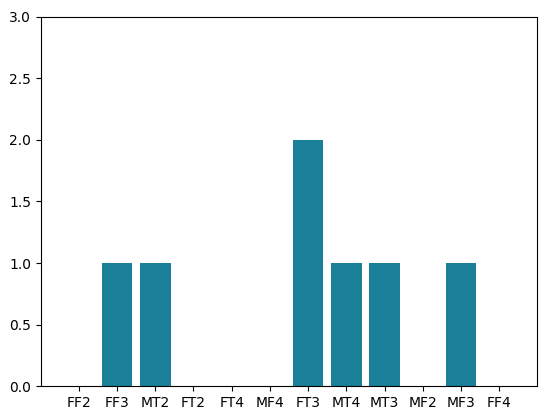
\includegraphics[height=4.5cm]{report-acceptance/PF-3.png} 
	\caption{Total of friend request accepted from \texttt{PF-3}}
	\label{fig:accepted-from-PF3}
\end{figure}
\par \noindent In detail, it can be noted that:
\begin{enumerate}
	\item it is accepted almost equally by men (4) and women (3);
	\item it is more accepted from those profiles with a real profile picture (5) than those with a false profile picture (2);
	\item it is accepted more by female profiles with the real profile picture (2) than with the false profile picture (1), like the male profiles where it is accepted by 3 profiles with the real profile picture and by only 1 with the false profile picture;
	\item it is accepted more by profiles over the age of 50 (5 in total, 3 women and 2 men) and equally by profiles aged between 18 and 50 (1 in total, 0 women and 1 man) and from profiles with hidden age (0 women and 1 man).
\end{enumerate}


\subsection*{PF-4}
It represents a \texttt{MF3} profile, that is a man aged over 50 and that in his Facebook profile he has the profile picture where he does not show his face.
\par \noindent The Figure \ref{fig:accepted-from-PF4} represents the collected data referred to this profile.
\begin{figure}[H]	
	\centering
	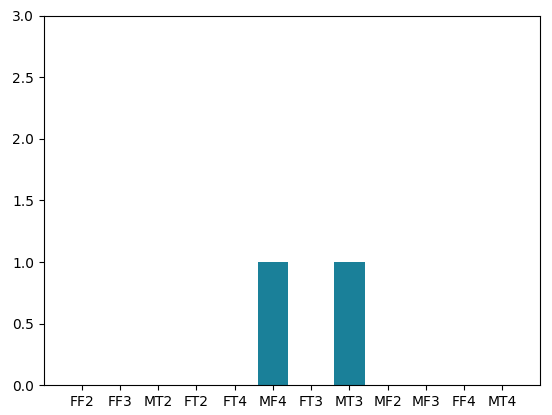
\includegraphics[height=4.5cm]{report-acceptance/PF-4.png} 
	\caption{Total of friend request accepted from \texttt{PF-4}}
	\label{fig:accepted-from-PF4}
\end{figure}
\par \noindent In detail, it can be noted that:
\begin{enumerate}
	\item it is accepted only by men (2) and by no one women (0), and this was the least accepted profile;
	\item it is accepted equally from profiles with a real profile picture (1) than those with a false profile picture (1);
	\item it was not accepted by female profiles with the real profile picture (0) and with the false profile picture (0), unlike the male profiles where it is accepted by 1 profile with the real profile picture and 1 with the false profile picture;
	\item it is accepted equally by profiles over the age of 50 (1 in total, 0 women and 2 men) and profiles with hidden age (0 women and 1 man), instead no one profile aged between 18 and 50 accepted the friend requests.
\end{enumerate}



\subsection*{PF-5}
It represents a \texttt{MT2} profile, that is a man aged between 18 and 50 and that in his Facebook profile he has the profile picture that shows his face.
\par \noindent The Figure \ref{fig:accepted-from-PF5} represents the collected data referred to this profile.
\begin{figure}[H]	
	\centering
	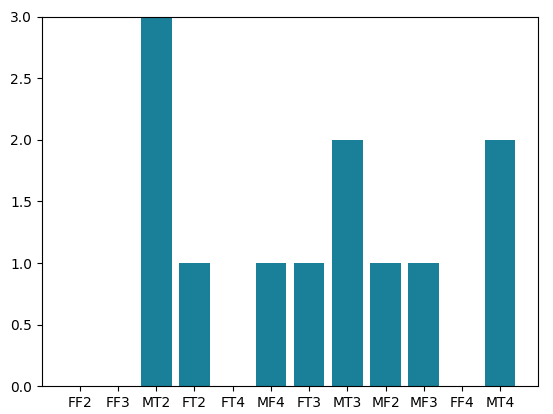
\includegraphics[height=4.5cm]{report-acceptance/PF-5.png} 
	\caption{Total of friend request accepted from \texttt{PF-5}}
	\label{fig:accepted-from-PF5}
\end{figure}
\par \noindent In detail, it can be noted that:
\begin{enumerate}
	\item it is more accepted from men (10) than women (2);
	\item it is more accepted from those with a real (9) profile picture than those profile with false (3) profile picture;
	\item it is accepted only by female profiles with the real profile picture (2 against 0 female profiles with false profile pictures), like the male profiles where it is accepted by 7 profiles with the real profile picture and by only 2 with the false profile picture;
	\item it is accepted more by profiles aged between 18 and 50 (5 in total, 1 woman and 4 men), followed by profiles over the age of 50 (4 in total, 1 woman and 3 men) and in the end it is accepted 3 times in total from profiles with hidden age (0 women and 3 man).
\end{enumerate}

\subsection*{PF-6}
It represents a \texttt{FT4} profile, that is a woman with hidden age and that in her Facebook profile she has the profile picture that shows her face.
\par \noindent The Figure \ref{fig:accepted-from-PF6} represents the collected data referred to this profile.
\begin{figure}[H]	
	\centering
	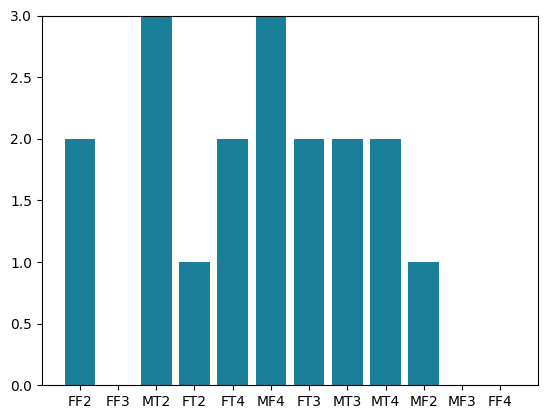
\includegraphics[height=4.5cm]{report-acceptance/PF-6.png} 
	\caption{Total of friend request accepted from \texttt{PF-6}}
	\label{fig:accepted-from-PF6}
\end{figure}
\par \noindent In detail, it can be noted that:
\begin{enumerate}
	\item it is more accepted from men (11) than women (7), and this was the most accepted profile;
	\item it is more accepted from those with a real (12) profile picture than those profile with false (6) profile picture;
	\item it is more accepted by female profiles with the real profile picture (5 against 2 female profiles with false profile pictures), like the male profiles where it is accepted by 7 profiles with the real profile picture and by 5 profiles with the false profile picture;
	\item it is accepted equally from profiles aged between 18 and 50 (7 in total, 3 women and 4 men) and from profiles with hidden age (2 women and 5 man), followed by profiles over the age of 50 (4 in total, 2 women and 2 men).
\end{enumerate}


\subsection*{PF-7}
It represents a \texttt{FF4} profile, that is a woman with hidden age and in her Facebook profile she has the profile picture where she does not show her face.
\par \noindent The Figure \ref{fig:accepted-from-PF7} represents the collected data referred to this profile.
\begin{figure}[H]	
	\centering
	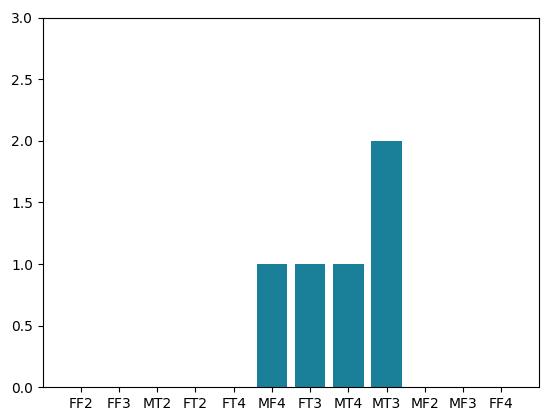
\includegraphics[height=4.5cm]{report-acceptance/PF-7.png} 
	\caption{Total of friend request accepted from \texttt{PF-7}}
	\label{fig:accepted-from-PF7}
\end{figure}
\par \noindent In detail, it can be noted that:
\begin{enumerate}
	\item it is more accepted from men (4) than women (1);
	\item it is more accepted from those with a real profile picture (4) than those have a false profile picture (1);
	\item it is accepted only by female profiles with the real profile picture (1 against 0 female profiles with false profile pictures), like the male profiles (1 had a false profile picture against 3 with a real profile picture);
	\item it is accepted more by profiles over the age of 50 (3 in total, 1 woman and 2 men) and followed by profiles aged between with hidden age (2 in total, 0 women and 2 men), while it was not accepted from profiles aged between 18 and 50 (0 women and 0 men).
\end{enumerate}


\subsection*{PF-8}
It represents a \texttt{FF2} profile, that is a woman aged between 18 and 50 and that in her Facebook profile she has the profile picture where she does not show her face.
\par \noindent The Figure \ref{fig:accepted-from-PF8} represents the collected data referred to this profile.
\begin{figure}[H]	
	\centering
	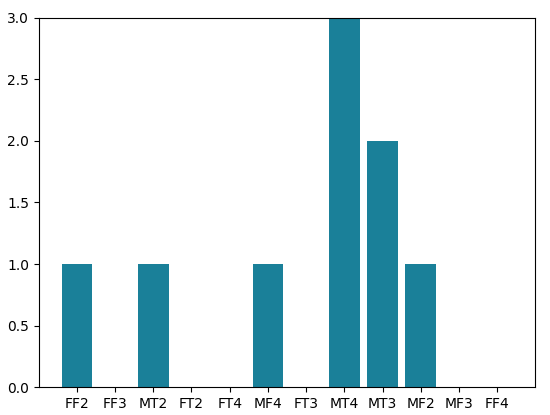
\includegraphics[height=4.5cm]{report-acceptance/PF-8.png} 
	\caption{Total of friend request accepted from \texttt{PF-8}}
	\label{fig:accepted-from-PF8}
\end{figure}
\par \noindent In detail, it can be noted that:
\begin{enumerate}		
	\item it is more accepted from men (8) than women (1);
	\item it is more accepted from those with a real profile picture (6) than those have a false profile picture (3);
	\item it is accepted only by female profiles with the false profile picture (1 against 0 female profiles with real profile pictures), unlike the male profiles (2 had a false profile picture against 6 with a real profile picture);
	\item it is accepted more by profiles with hidden age (4 in total, 0 women and 4 men) and followed by profiles aged between 18 and 50 (3 in total, 1 woman and 2 men), while it is accepted only twice from profiles over the age of 50 (0 women and 2 men).
\end{enumerate}


\subsection*{PF-9}
It represents a \texttt{FT3} profile, that is a woman aged between 18 and 50 and that in her Facebook profile she has the profile picture where she does not show her face.
\par \noindent The Figure \ref{fig:accepted-from-PF9} represents the collected data referred to this profile.
\begin{figure}[H]	
	\centering
	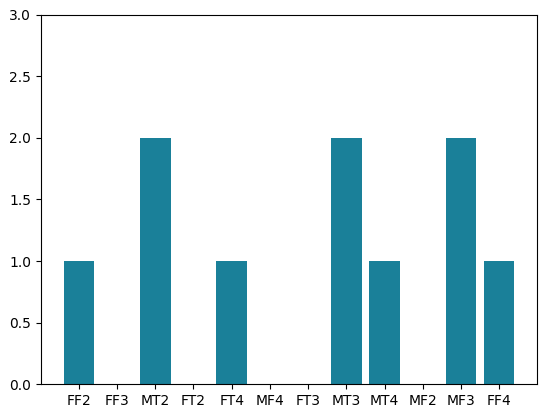
\includegraphics[height=4.5cm]{report-acceptance/PF-9.png} 
	\caption{Total of friend request accepted from \texttt{PF-9}}
	\label{fig:accepted-from-PF9}
\end{figure}
\par \noindent In detail, it can be noted that:
\begin{enumerate}		
	\item it is more accepted from men (7) than women (3);
	\item it is more accepted from those with a real profile picture (6) than those have a false profile picture (4);
	\item it is more accepted by female profiles with the false profile picture (2 against 1 female profiles with real profile pictures), unlike the male profiles (2 had a false profile picture against 5 with a real profile picture);
	\item it was accepted more by profiles over the age of 50 (4 in total, 0 women and 4 men) and followed by profiles aged between 18 and 50 (3 in total, 1 woman and 2 men) on a par with profiles with hidden age (3 in total, 2 women and 1 man).
\end{enumerate}


\subsection*{PF-10}
It represents a \texttt{FF3} profile, that is a woman aged over 50 and that in her Facebook profile she has the profile picture where she does not show her face.
\par \noindent The Figure \ref{fig:accepted-from-PF10} represents the collected data referred to this profile.
\begin{figure}[H]	
	\centering
	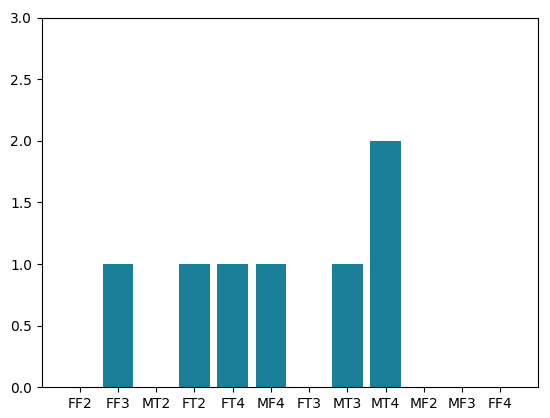
\includegraphics[height=4.5cm]{report-acceptance/PF-10.png} 
	\caption{Total of friend request accepted from \texttt{PF-10}}
	\label{fig:accepted-from-PF10}
\end{figure}
\par \noindent In detail, it can be noted that:
\begin{enumerate}		
	\item it is accepted almost equally from men (4) and women (3);
	\item it is more accepted from those with a real profile picture (5) than those have a false profile picture (2);
	\item it is more accepted by female profiles with the real profile picture (2 against 1), like the male profiles (3 against 1);
	\item it was accepted more by profiles over the hidden age (4 in total, 1 woman and 3 men), followed by profiles over the age of 50 (2 in total, 1 woman and 1 man) and by profiles aged between 18 and 50  (3 in total, 2 women and 1 man).
\end{enumerate}


\subsection*{PF-11}
It represents a \texttt{FT2} profile, that is a woman aged between 18 and 50 and that in her Facebook profile she has the profile picture that shows her face.
\par \noindent The Figure \ref{fig:accepted-from-PF11} represents the collected data referred to this profile.
\begin{figure}[H]	
	\centering
	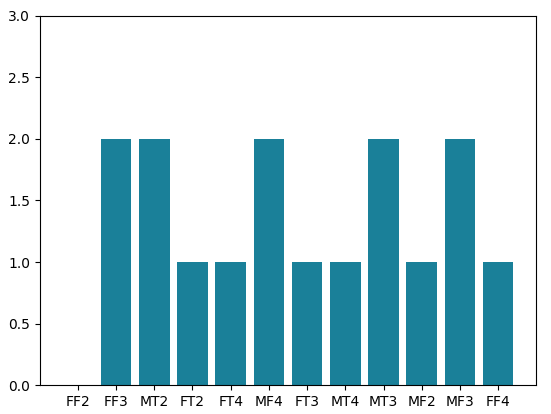
\includegraphics[height=4.5cm]{report-acceptance/PF-11.png} 
	\caption{Total of friend request accepted from \texttt{PF-11}}
	\label{fig:accepted-from-PF11}
\end{figure}
\par \noindent In detail, it can be noted that:
	\begin{enumerate}		
	\item it is more accepted from men (10) than women (6);
	\item it is accepted equally by both those with a real (8) and a false (8) profile picture;
	\item it is accepted equally by female profiles with a real (3) and a false (3) profile picture, like the male profiles (both cases with 5);
	\item it is accepted more by profiles over the age of 50 (7 in total, 3 women and 4 men), followed by profiles with hidden age (5 in total, 2 women and 3 men), and in the end it is only accepted 4 times in total from profiles aged between 18 and 50 (1 woman and 3 men).
\end{enumerate}

\newpage
%********************************************************************************%
\newpage
\section{Model of acceptance}
\subsection{The tool}
\label{cap:model-of-acceptance}
With a tool, called \texttt{acceptance\_model.py}, which analize the content of \\ \texttt{distribution\_update.json} dataset (details in \ref{cap:distribution-update}), an acceptance model will be created.
\par \noindent
The tool, run from the terminal, requires the \texttt{distribution\_update.json} dataset and for each type of victim, it analyze and describes the acceptance rate of every type of attacker profile. Considering that the number of friend requests from an attacker profile to each type of victim profile is ``3'', an attacker profile could have 4 types of probability, based on the number of how many friend requests from that attacker profile that type of victim have accepted:
\begin{itemize}
	\item the acceptance rate is \texttt{0/3}, if no one has been accepted the friend requests;
	\item the acceptance rate is \texttt{1/3}, if it has been accepted only one;
	\item the acceptance rate is \texttt{2/3}, if two requests have been accepted;
	\item the acceptance rate is \texttt{3/3}, if all requests have been accepted.
\end{itemize}
For each victim the result that the tool shows in the terminal will be discussed in the next section.
\subsection{The model}
This section discusses the acceptance model resulting from the execution of the \texttt{acceptance\_model.py} tool after the last one collection and analysis of the data on 6th September.
\par \noindent
The Figure \ref{fig:model-screen} shows a portion of the output of the \texttt{acceptance\_model.py} tool, with a part of the representation of the acceptance model.
\label{cap:model-acceptance}
\begin{figure}[H]	
	\centering
	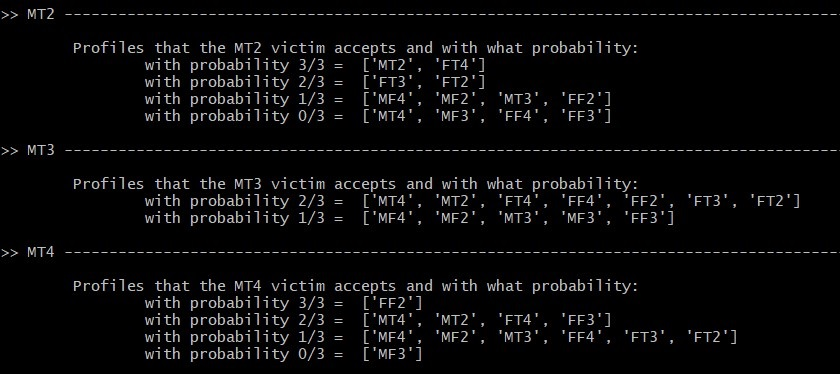
\includegraphics[height=5.5cm]{immagini/model-zero-effort.jpg}
	\caption{Screen of the model of accepatance shows by the \texttt{acceptance\_model.py} tool}
	\label{fig:model-screen}
\end{figure}
\newpage
\par \noindent
The Table \ref{table:ranking-victim} shows a ranking starting from the victim who accepted the most friend requests, up to the one who accepted the least number of friend requests.

\begin{table}[H]
	\begin{center}
		\begin{tabular}[c]{ |c|c|c| } 
			\hline
			\cellcolor[HTML]{b0d7ff}\textsc{position} & 
			\cellcolor[HTML]{b0d7ff}\textsc{label}& 
			\cellcolor[HTML]{b0d7ff}\textsc{ranking}\\
			%\cellcolor[HTML]{e6f2ff}
			\hline 
			\textbf{\textsc{1°}}
			&\cellcolor[HTML]{e6f2ff}\texttt{MT3}
			& \texttt{52,25\%}\\	 
			\hline
			\textbf{\textsc{2°}}
			&\cellcolor[HTML]{e6f2ff}\texttt{MT4}
			& \texttt{44,44\%}\\	 
			\hline
			\textbf{\textsc{3°}}
			&\cellcolor[HTML]{e6f2ff}\texttt{MT2}
			& \texttt{46,83\%}\\	 
			\hline
			\textbf{\textsc{4°}}
			&\cellcolor[HTML]{e6f2ff}\texttt{MF4}
			& \texttt{36,00\%}\\	 
			\hline
			\textbf{\textsc{5°}}
			&\cellcolor[HTML]{e6f2ff}\texttt{MF3}
			& \texttt{25,25\%}\\	 
			\hline
			\textbf{\textsc{6°}}
			&\cellcolor[HTML]{e6f2ff}\texttt{FT3}
			& \texttt{25,17\%}\\	 
			\hline			
			\textbf{\textsc{7°}}
			&\cellcolor[HTML]{e6f2ff}\texttt{FT4}
			& \texttt{22,50\%}\\	 
			\hline			
			\textbf{\textsc{8°}}
			&\cellcolor[HTML]{e6f2ff}\texttt{MF2}
			& \texttt{19,75\%}\\	 
			\hline			
			\textbf{\textsc{9°}}
			&\cellcolor[HTML]{e6f2ff}\texttt{FF3}
			& \texttt{17,17\%}\\	 
			\hline
			\textbf{\textsc{10°}}
			&\cellcolor[HTML]{e6f2ff}\texttt{FF2}
			& \texttt{14,42\%}\\	 
			\hline
			\textbf{\textsc{11°}}
			&\cellcolor[HTML]{e6f2ff}\texttt{FT2}
			& \texttt{14,33\%}\\	 
			\hline
			\textbf{\textsc{12°}}
			&\cellcolor[HTML]{e6f2ff}\texttt{FF4}
			& \texttt{6,33\%}\\	 
			\hline
		\end{tabular}
	\end{center}
	\caption{Victim profiles ranking.}
	\label{table:ranking-victim}
\end{table}

\par \noindent The acceptance model for each victim is now discussed and argued.

\subsection*{FF2 victim}
"\texttt{FF2}" means that the victim is a woman aged between 18 and 50 and that in her Facebook profile she has the profile picture where she does not show her face.
From the model the profiles that the FF2 victim accepts:
\begin{itemize}
	\item with probability \texttt{2/3} $\rightarrow$ \texttt{FT4},
	\item with probability \texttt{1/3} $\rightarrow$ \texttt{FF2, FT3, MF2}.
\end{itemize}  
All other attacker profiles have a \texttt{0/3} chance of being accepted.
\par \noindent In this circumstance it can be seen that, as learned in the previous chapters, women are less inclined to accept the friend request. Furthermore, this profile easily accepts only \texttt{4} types of profiles, \texttt{3} of which are female.
\par \noindent In a ranking starting from the victim who accepted the most friend requests up to the one who accepted the least number of friend requests, it ranks 10th place with \textbf{14,42\%}.


\subsection*{FF3 victim}
"\texttt{FF3}" means that the victim is a woman aged over 50 and that in her Facebook profile she has the profile picture where she does not show her face.
From the model the profiles that the FF3 victim accepts:
\begin{itemize}
	\item with probability \texttt{2/3} $\rightarrow$ \texttt{FT2, MT4},
	\item with probability \texttt{1/3} $\rightarrow$ \texttt{FF3, MT3}.
\end{itemize}  
All other attacker profiles have a \texttt{0/3} chance of being accepted.
\par \noindent In this case we notice how this victim tends to accept profiles with the real profile image more easily, probably because he can have a clearer idea of who he is in front of: \texttt{3/4} of the accepted profiles have in fact the real profile image.
\par \noindent In a ranking starting from the victim who accepted the most friend requests up to the one who accepted the least number of friend requests, it ranks 9th place with \textbf{17,17\%}.


\subsection*{FF4 victim}
"\texttt{FF4}" means that the victim is a woman with hidden age and in her Facebook profile she has the profile picture where she does not show her face.
From the model the profiles that the FF4 victim accepts:
\begin{itemize}
	\item with probability \texttt{1/3} $\rightarrow$ \texttt{FT2, FT3}.
\end{itemize}  
All other attacker profiles have a \texttt{0/3} chance of being accepted.
\par \noindent This is the profile that protects itself the most and therefore does not easily accept friend requests. Age is hidden, so it could be an underage girl as well as a very adult lady. This profile wants safety first of all and accepts only female profiles and with visible age.
\par \noindent In a ranking starting from the victim who accepted the most friend requests up to the one who accepted the least number of friend requests, it ranks in the lowest point of the ranking, precisely in 12th place, with \textbf{6.33\%}.


\subsection*{FT2 victim}
"\texttt{FT2}" means that the victim is a woman aged between 18 and 50 and that in her Facebook profile she has the profile picture that shows her face.
From the model the profiles that the FT2 victim accepts:
\begin{itemize}
	\item with probability \texttt{1/3} $\rightarrow$ \texttt{MT4, MT2, FT4, FF3, FT2}.
\end{itemize}  
All other attacker profiles have a \texttt{0/3} chance of being accepted.
\par \noindent Also in this circumstance it can be seen that women are more difficult to accept a friend request: this profile has a very low success rate due to the fact that the greater probability is only 1/3 and that the profiles that enjoy this probability are the 40\% of the total (5 profiles out of 12 total).
\par \noindent In a ranking starting from the victim who accepted the most friend requests up to the one who accepted the least number of friend requests, it ranks 11th place with \textbf{14.33\%}.


\subsection*{FT3 victim}
"\texttt{FT3}" means that the victim is a woman aged over 50 and that in her Facebook profile she has the profile picture that shows her face.
From the model the profiles that the FT3 victim accepts:
\begin{itemize}
	\item with probability \texttt{2/3} $\rightarrow$ \texttt{FT4, MT3},
	\item with probability \texttt{1/3} $\rightarrow$ \texttt{MT4, MF4, MT2, FF4, FT2}.
\end{itemize}  
All other attacker profiles have a \texttt{0/3} chance of being accepted.
\par \noindent In this case it can be verified that a profile with the image of the real profile is accepted more easily, as learned in the previous chapters: 5 out of 7 total accepted profiles, have the image of the real profile.
\par \noindent In a ranking starting from the victim who accepted the most friend requests up to the one who accepted the least number of friend requests, it ranks 6th with \textbf{25.17\%}.


\subsection*{FT4 victim}
"\texttt{FT4}" means that the victim is a woman with hidden age and that in her Facebook profile she has the profile picture that shows her face.
From the model the profiles that the FT4 victim accepts:
\begin{itemize}
	\item with probability \texttt{2/3} $\rightarrow$ \texttt{FT4, MT4},
	\item with probability \texttt{1/3} $\rightarrow$ \texttt{MF4, FT3, FF3, FT2}.
\end{itemize}  
All other attacker profiles have a \texttt{0/3} chance of being accepted.
\par \noindent Also in this case you can see how the profiles of women are more accepted than the profiles of men, especially if the profile picture is showing the person's face. We can also note that half of the accepted profiles have the hidden age, exactly like the victim: this could be because the victim, having herself the hidden age, understands that age is a very personal factor that some people hardly show publicly and therefore tends to trust people who act like her.
\par \noindent In a ranking starting from the victim who accepted the most friend requests up to the one who accepted the least number of friend requests, it ranks 7th with \textbf{22.50\%}.


\subsection*{MF2 victim}
\texttt{MF2} means that the victim is a man aged between 18 and 50 and that in his Facebook profile he has the profile picture that does not show his face.
From the model the profiles that the MF2 victim accepts:
\begin{itemize}
	\item with probability \texttt{2/3} $\rightarrow$ \texttt{MT4},
	\item with probability \texttt{1/3} $\rightarrow$ \texttt{MF4, MT2, FT4, FF2, FT2}.
\end{itemize}  
All other attacker profiles have a \texttt{0/3} chance of being accepted.
\par \noindent In this particular case it can be seen how this victim tends to accept mainly profiles with the same age range (3/6) and with the real profile image (4/6).
\par \noindent In a ranking starting from the victim who accepted the most friend requests up to the one who accepted the least number of friend requests, it ranks 8th with \textbf{19.75\%}.


\subsection*{MF3 victim}
"\texttt{MF3}" means that the victim is a man aged over 50 and that in his Facebook profile he has the profile picture where he does not show his face.
From the model the profiles that the MF3 victim accepts:
\begin{itemize}
	\item with probability \texttt{2/3} $\rightarrow$ \texttt{MF2, FT3, FT2},
	\item with probability \texttt{1/3} $\rightarrow$ \texttt{MT4, MT3, MT2}.
\end{itemize}  
All other attacker profiles have a \texttt{0/3} chance of being accepted.
From this study it can be deduced that the only attention that the victim pays when he finds a friend request is in the profile image: in fact all the profiles that he has not accepted have the profile image that is not real. This profile therefore wants to protect himself by putting a profile picture that does not show his face, but at the same time does not trust anyone who does not have the real image.
\par \noindent In a ranking starting from the victim who accepted the most friend requests up to the one who accepted the least number of friend requests, it ranks \texttt{5th} place with \textbf{25.25\%}.


\subsection*{MF4 victim}
"\texttt{MF4}" means that the victim is a man with hidden age and that in his Facebook profile he has the profile picture where he does not show his face.
From the model the profiles that the MF4 victim accepts:
\begin{itemize}
	\item with probability \texttt{3/3} $\rightarrow$ \texttt{FT4},	
	\item with probability \texttt{2/3} $\rightarrow$ \texttt{MT4, FT2},
	\item with probability \texttt{1/3} $\rightarrow$ \texttt{MF4, MF3, MT2, FF4, FF2, FF3}.
\end{itemize}  
All other attacker profiles have a \texttt{0/3} chance of being accepted. \par \noindent
This victim has no particular attention as to who to accept the friendship. He accepts both males and females equally, with both real and non-real images. The only highlight: this is one of the few types of victim who has accepted at least one request to each profile with the hidden age. Maybe it's because he hides his age too and, as in the case of the FT4 profile, he thinks of age as a very personal factor that some people hardly show publicly and therefore tends to trust people who behave like him.
\par \noindent In a ranking starting from the victim who accepted the most friend requests up to the one who accepted the least number of friend requests, it ranks \texttt{4th} place with \textbf{36.00\%}.


\subsection*{MT2 victim}
"\texttt{MT2}" means that the victim is a man aged between 18 and 50 and that in his Facebook profile he has the profile picture that shows his face.
From the model the profiles that the MT2 victim accepts:
\begin{itemize}
	\item with probability \texttt{3/3} $\rightarrow$ \texttt{MT2, FT4},	
	\item with probability \texttt{2/3} $\rightarrow$ \texttt{FT3, FT2},
	\item with probability \texttt{1/3} $\rightarrow$ \texttt{MF4, MF2, MT3, FF2}.
\end{itemize} 
All other attacker profiles have a \texttt{0/3} chance of being accepted. \par \noindent
This victim has no particular attention on who to accept friendship: she accepts both males and females equally, preferring those with the real profile image (5/8) and avoiding (especially among profiles with a non-real profile image ) that report an older or hidden age.
\par \noindent In a ranking starting from the victim who accepted the most friend requests up to the one who accepted the least number of friend requests, it ranks \texttt{3rd} place with \textbf{38.83\%}.


\subsection*{MT3 victim}
"\texttt{MT3}" means that the victim is a man aged between over 50 and that in his Facebook profile he has the profile picture that shows his face.
From the model the profiles that the MT2 victim accepts:
\begin{itemize}
	\item with probability \texttt{2/3} $\rightarrow$ \texttt{MT4, MT2, FT4, FF4, FF2, FT3, FT2},
	\item with probability \texttt{1/3} $\rightarrow$ \texttt{MF4, MF2, MT3, MF3, FF3}.
\end{itemize} 
No one attacker profiles have a \texttt{0/3} chance of being accepted. \par \noindent
This victim has no particular focus on who to accept the friendship: he is the only type of profile that has accepted all kinds of requests from all kinds of attackers. If you want to target this type of victim, the profile to be created is almost irrelevant what characteristics it has. The only caution is that she accepts more female profiles, regardless of age.
\par \noindent In a ranking starting from the victim who accepted the most friend requests up to the one who accepted the least number of friend requests, it ranks in the highest point of the ranking, in \texttt{1st} place, with \textbf{52.25\%}.


\subsection*{MT4 victim}
"\texttt{MT4}" means that the victim is a man with hidden age and that in his Facebook profile he has the profile picture that shows his face.
From the model the profiles that the MT4 victim accepts:
\begin{itemize}
	\item with probability \texttt{3/3} $\rightarrow$ \texttt{FF2},
	\item with probability \texttt{2/3} $\rightarrow$ \texttt{MT4, MT2, FT4, FF3},
	\item with probability \texttt{1/3} $\rightarrow$ \texttt{MF4, MF2, MT3, FF4, FT3, FT2}.
\end{itemize} 
Only \texttt{MF3} attacker profiles have a \texttt{0/3} chance of being accepted. \par \noindent
Like \texttt{MT3}, this victim has no particular focus on who to accept friendship: with the exception of the \texttt{MF3} profile, she has accepted all kinds of requests from all kinds of attackers. Always like the \texttt{MT3} profile, the profile to be created to target this victim, the only precaution could be to create a profile of a woman.
\par \noindent In a ranking starting from the victim who accepted the most friend requests up to the one who accepted the least number of friend requests, it ranks \texttt{2nd} place with \textbf{46.83\%}.

\newpage
\section{Zero-Effort Attack}
\label{cap:zero-effort-attack}
``\texttt{Zero-Effort Attack}'' is the name of the final tool. This was the goal of the internship. Its name is derived from the effective effort that the attacker gonna do, i.e., \texttt{zero}. That's because the attacker must enter the URL of the victim profile on the terminal and the tool will show in the output the model of acceptance (Chapter \ref{cap:model-acceptance}) for that type of victim.
\par \noindent In detail, the tool, run from the terminal, requires as input:
\begin{itemize}
	\item \texttt{email},\par \noindent the email that the attacker use to log into Facebook.\par \noindent Accepted values: string parameter (\texttt{string});
	
	\item \texttt{pwd},\par \noindent the password that the attacker use to log into Facebook.\par \noindent Accepted values: string parameter (\texttt{string});
	
	\item \texttt{url},\par \noindent the URL of victim profile to attack.\par \noindent Accepted values: string parameter (\texttt{string});
\end{itemize}
This tool get the \texttt{email} and \texttt{password} parameters to log into Facebook. After that, it goes to the page of the victim profile thanks to the \texttt{URL} parameter.
Now the tool can analyze the victim, and the procedure is the same as the \texttt{classificator-profile} tool (Chapter \ref{cap:classificator-profiles}).
\par \noindent Once the victim's profile has been analyzed, it categorizes it by assigning it the corresponding label. With that label, the tool will examine the acceptance model and show in the terminal which type of attacker profiles are accepted and with what probability.
\par \noindent Then the tool asks the attacker to choose the type of a victim profile to create. The attacker enters the label (and the tool checks that the label exists but not the acceptance rate) and the tool show a false profile: with the same procedure of the \texttt{create-profile.py} tool (Chapter \ref{cap:tool-create}) and based on the label of the victim profile chosen by the attacker, it selects a name, a surname, an existent date of birth and how to set the profile picture. It also proposes a work occupation and a current town insert in the Facebook profile. The working occupation value is random but the current town is based on the current town of the victim: if it is visible, the tool suggests setting the current town near the victim town, if it is not visible, it suggests nothing. This case of study does not consider these parameters (but they could be a future development as mentioned in Chapter \ref{cap:town-occupation}), but they are indicated to favor the creation of a complete profile.
\par \noindent
In the end, the tool asks the attacker to approve (or not) the suggested fake profile. In case the attacker is not convinced by the suggested profile, he can ask that the tool show him another one, until he gets one of his likings.
\par \noindent
The Figure \ref{fig:zero-effort-tool} displays what the terminal show in the output to the attacker at the end of the procedure.

\begin{figure}[H]
	\centering
	\caption{An example of the execution of the \texttt{zero-effort-attack.py} tool from the terminal.}
	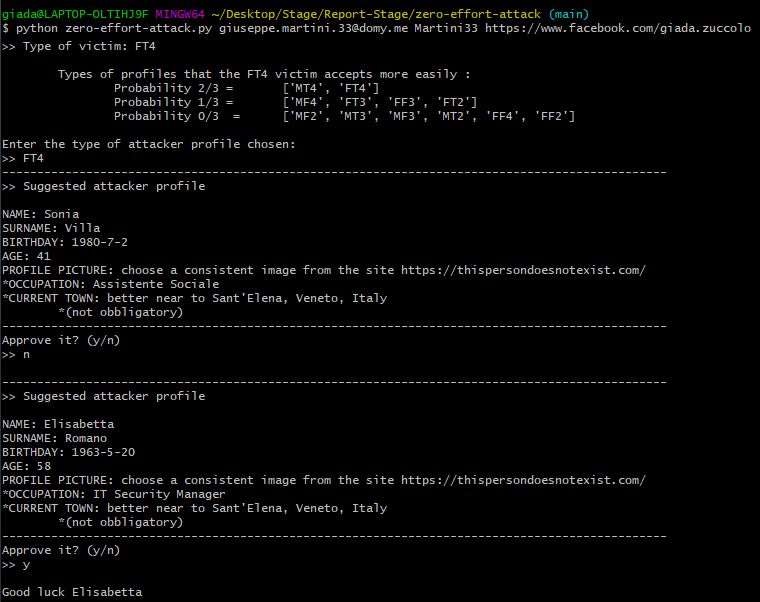
\includegraphics[height=11cm]{immagini/zero-effort-exe.png} 
	\label{fig:zero-effort-tool}
\end{figure}